\documentclass[12pt,a4paper]{article}
\usepackage{ctex}
\usepackage{amsmath,amssymb}
\usepackage{graphicx}
\usepackage{float}
\usepackage{listings}
\usepackage{xcolor}
\usepackage{geometry}
\usepackage{fancyhdr}
\usepackage{tocbibind} % 显示目录
\usepackage{tikz}      % 画流程图
\usepackage{hyperref}

% 页面设置
\geometry{left=2.5cm,right=2.5cm,top=2.8cm,bottom=2.5cm}
\setlength{\headheight}{15pt}

% MATLAB代码样式
\lstset{
    language=Matlab,
    basicstyle=\ttfamily\small,
    keywordstyle=\color{blue},
    commentstyle=\color{green!70!black},
    stringstyle=\color{red},
    numbers=left,
    numberstyle=\tiny,
    frame=single,
    breaklines=true,
    backgroundcolor=\color{gray!5}
}

% 页眉页脚
\pagestyle{fancy}
\fancyhf{}
\lhead{信号分析与处理实验报告}
\rhead{\thesection}
\cfoot{\thepage}

% 超链接样式（无红框）
\hypersetup{
    colorlinks=true,
    linkcolor=blue,
    citecolor=blue,
    urlcolor=blue
}

\begin{document}

% 封面
\begin{center}
    \vspace*{2cm}
    {\Huge \textbf{信号分析与处理实验报告}}\\[2cm]
    
    \Large
    姓\quad\quad 名：\textbf{余泓彬} \\[1em]
    学\quad\quad 号：\textbf{2024312506} \\[1em]
    班\quad\quad 级：\textbf{电气1班} \\[3cm]
\end{center}

\newpage

% 目录
\tableofcontents
\newpage

% 导入实验
\section{实验一 周期信号的分解与合成}
\subsection{一、实验流程图}
\begin{figure}[H]
\centering
\begin{tikzpicture}[
    node distance=1.6cm,
    auto,
    block/.style={rectangle, draw, text width=8.5em, align=center, minimum height=2.8em}
]
\node [block] (start) {程序初始化};
\node [block,below of=start] (para) {设置信号参数};
\node [block,below of=para] (gen) {生成原始周期信号};
\node [block,below of=gen] (fs) {傅里叶级数合成};
\node [block,below of=fs] (dfs) {离散 DFS/IDFS 分析};
\node [block,below of=dfs] (plot) {绘制波形与频谱};
\node [block,below of=plot] (end) {结束};

\draw[->] (start) -- (para);
\draw[->] (para) -- (gen);
\draw[->] (gen) -- (fs);
\draw[->] (fs) -- (dfs);
\draw[->] (dfs) -- (plot);
\draw[->] (plot) -- (end);
\end{tikzpicture}
\caption{实验一程序流程图}
\end{figure}

\subsection{二、实验结果附图}
\begin{figure}[H]
\centering
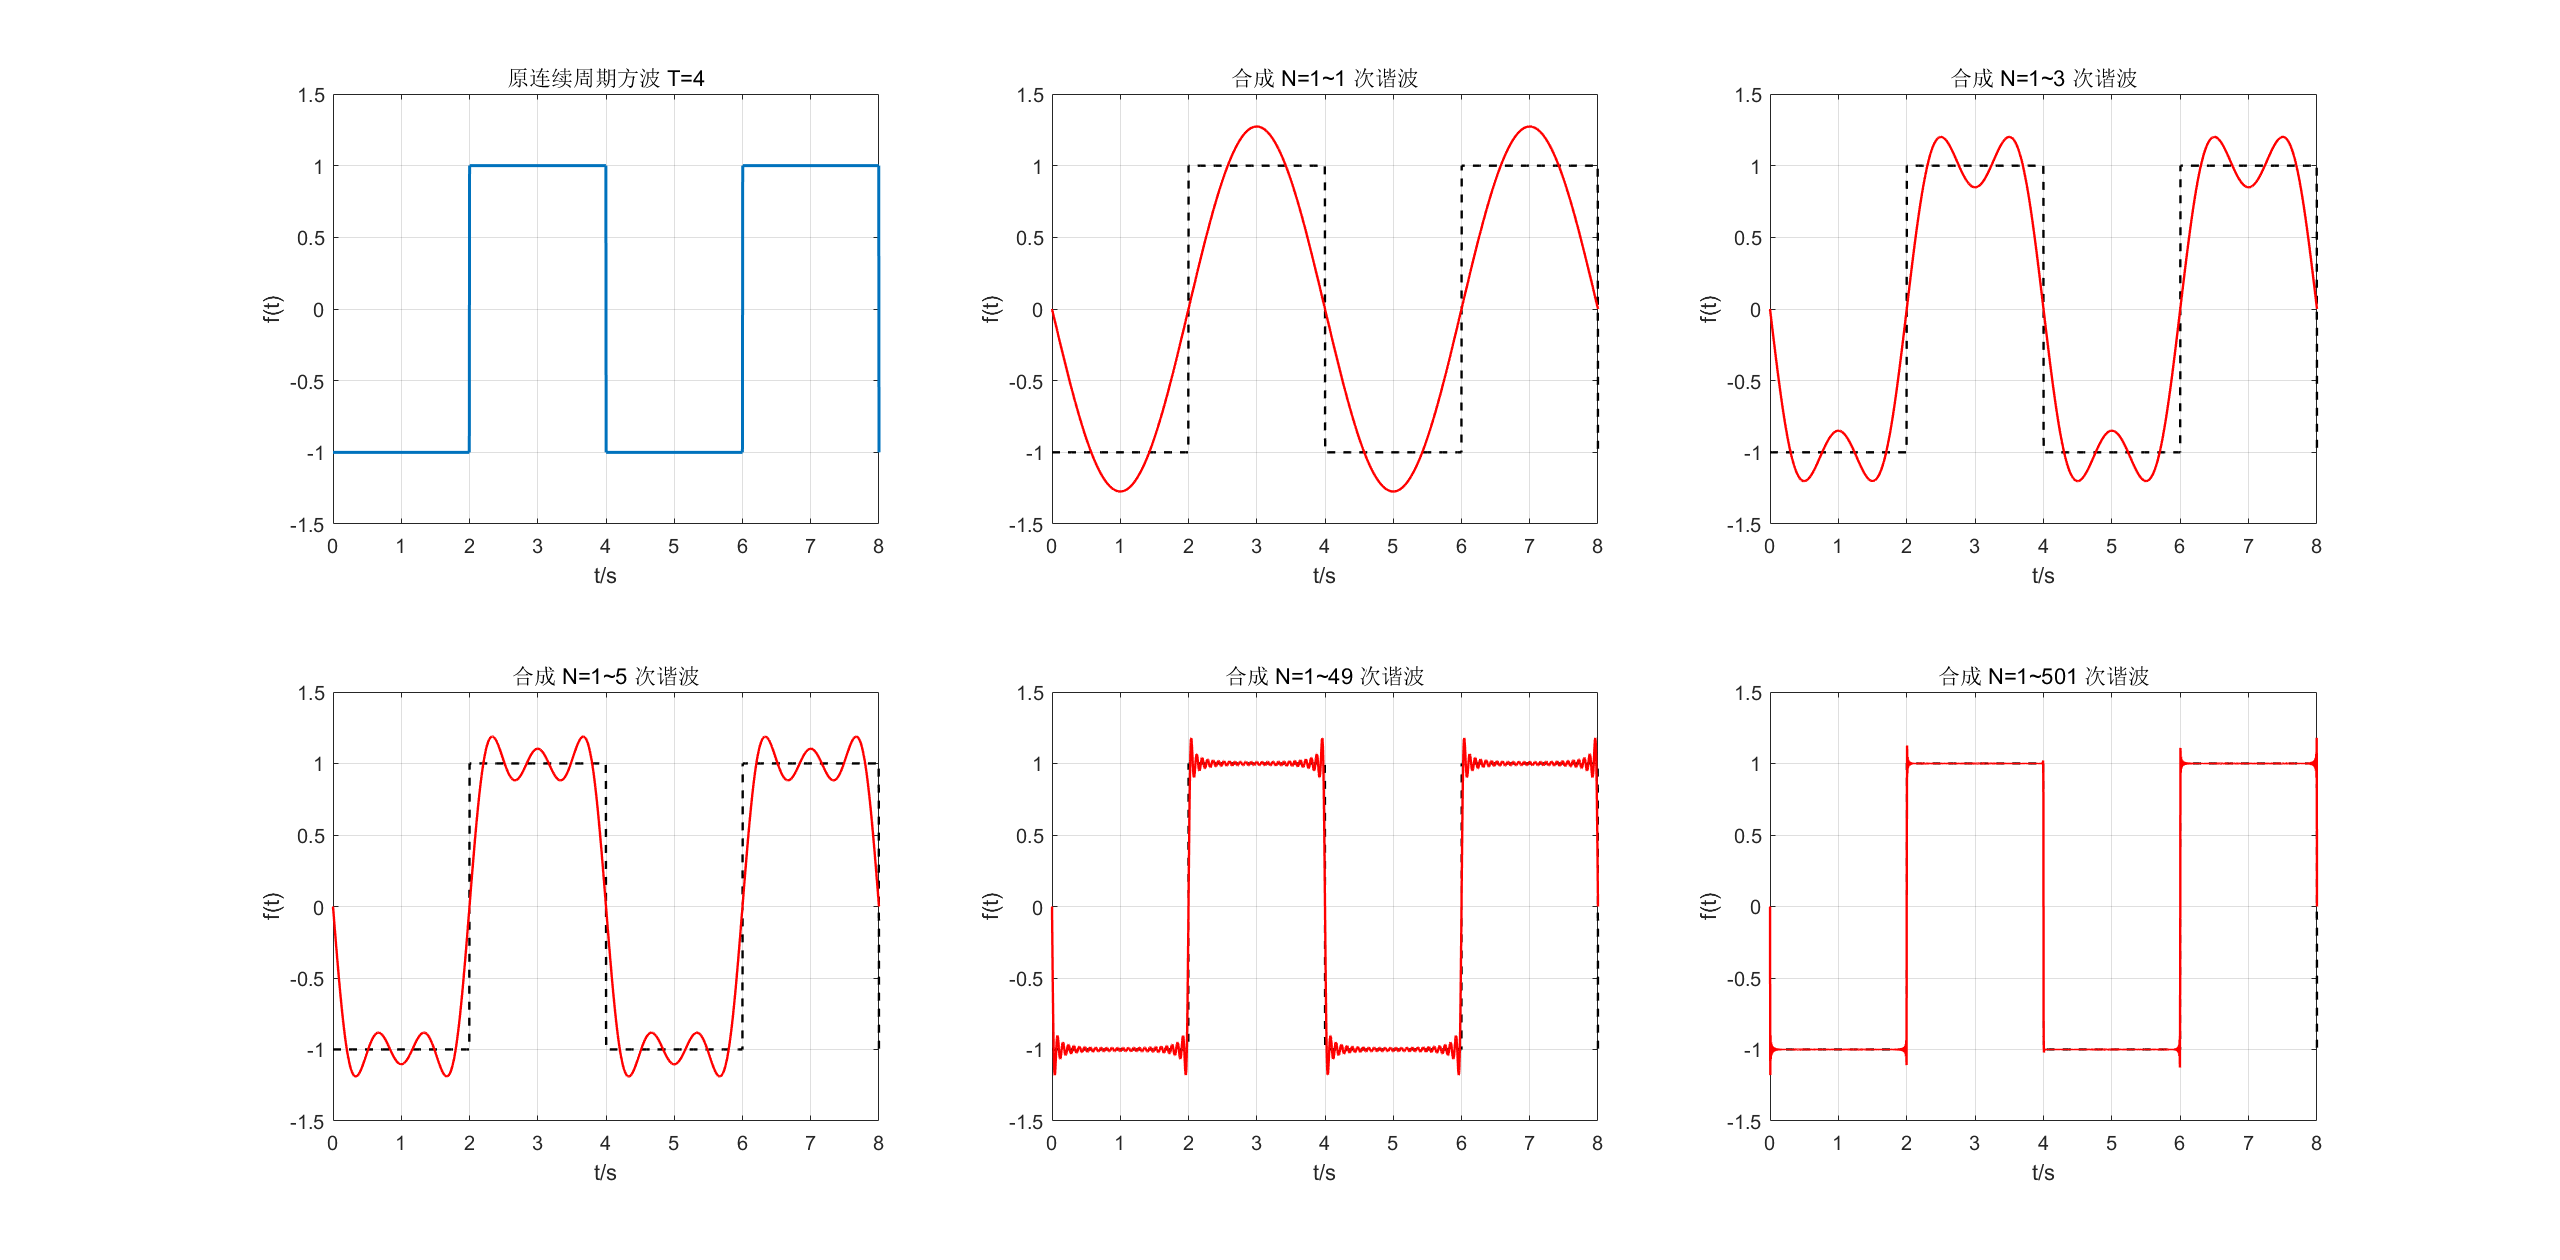
\includegraphics[width=0.8\textwidth]{1.1.png}
\caption{连续周期方波原始时域波形}
\end{figure}

\begin{figure}[H]
\centering
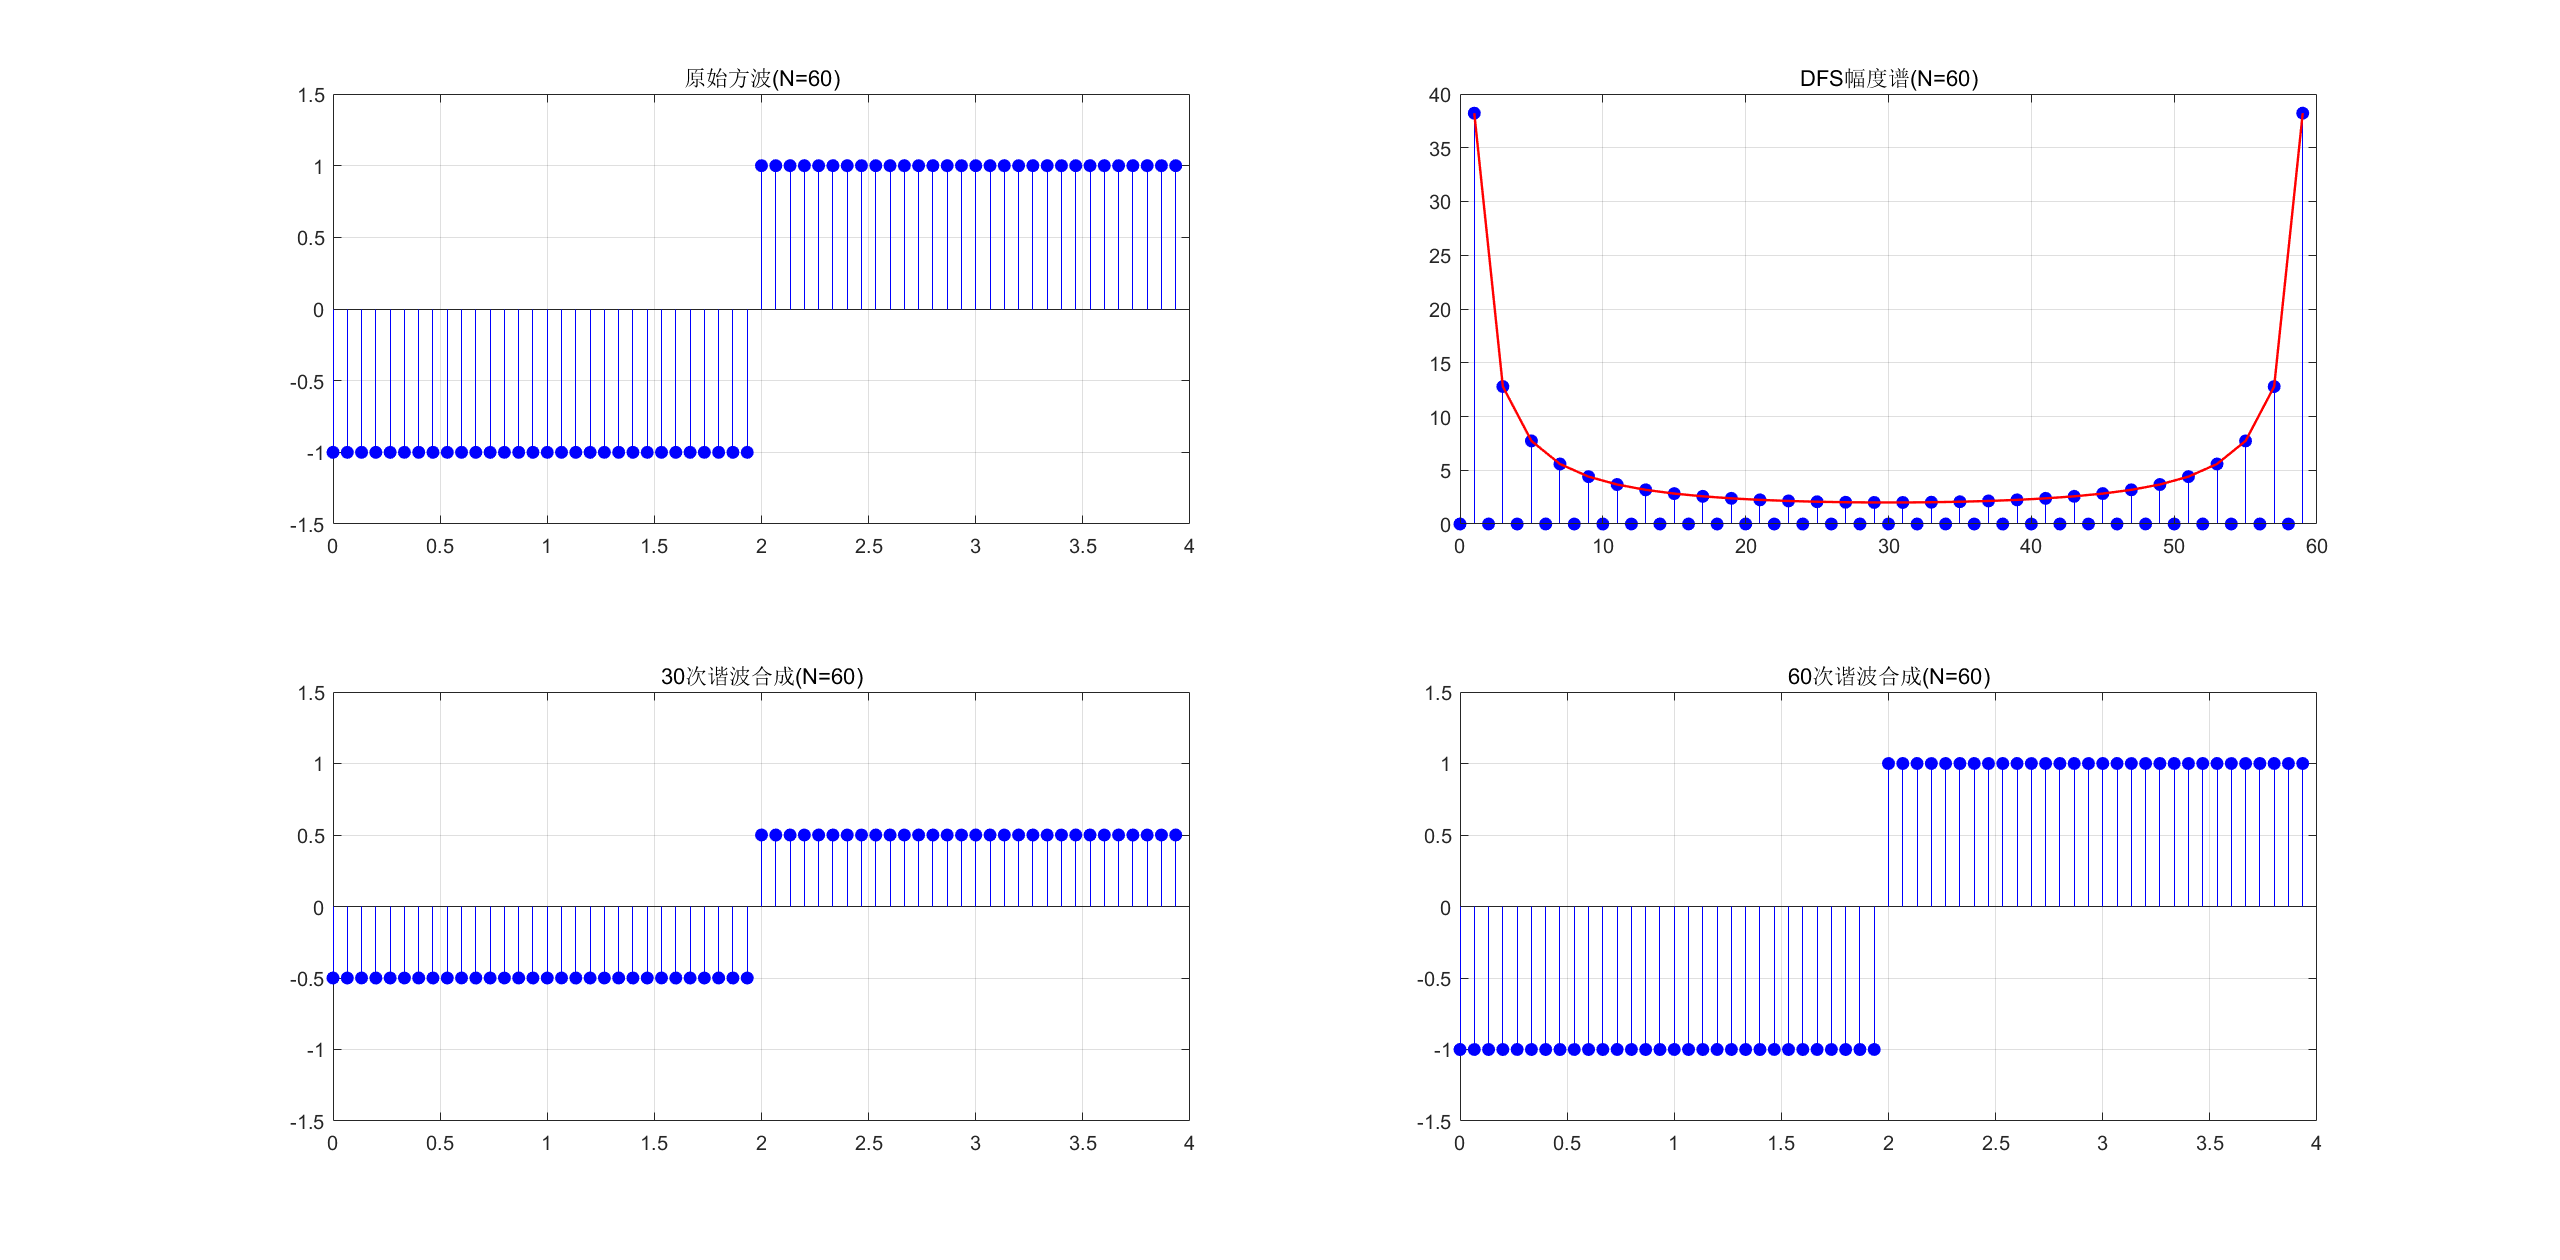
\includegraphics[width=0.8\textwidth]{1.2.1.png}
\caption{1次、1+3+5次谐波叠加波形对比}
\end{figure}

\begin{figure}[H]
\centering
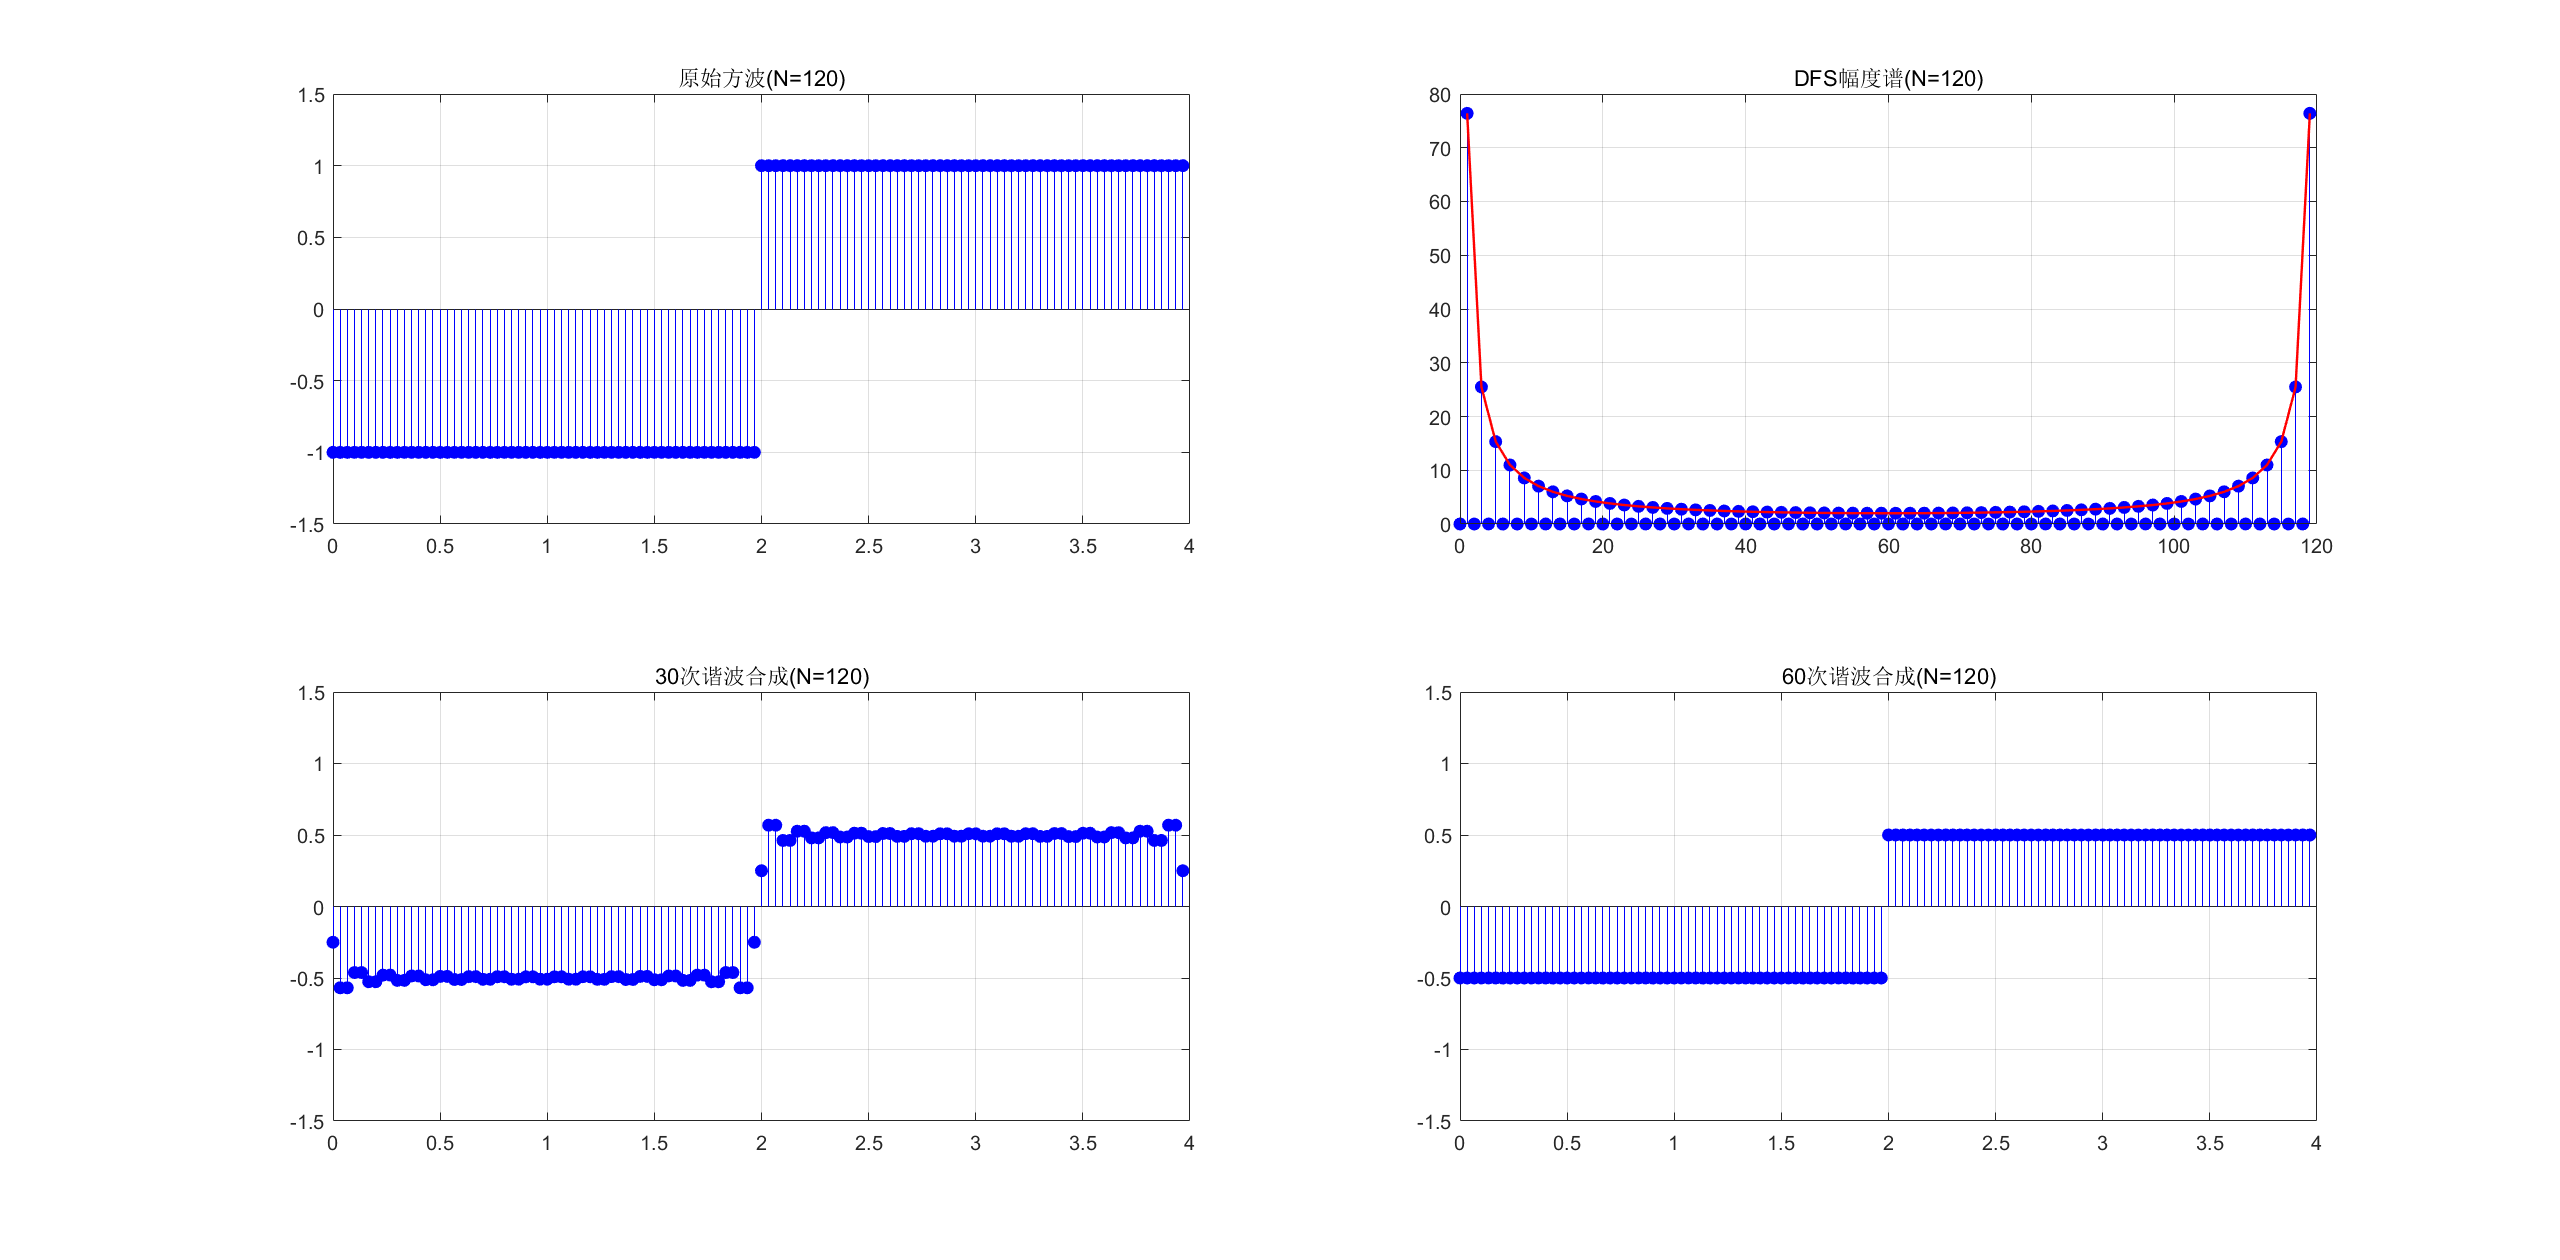
\includegraphics[width=0.8\textwidth]{1.2.2.png}
\caption{49次、501次谐波叠加（吉布斯现象）}
\end{figure}

\begin{figure}[H]
\centering
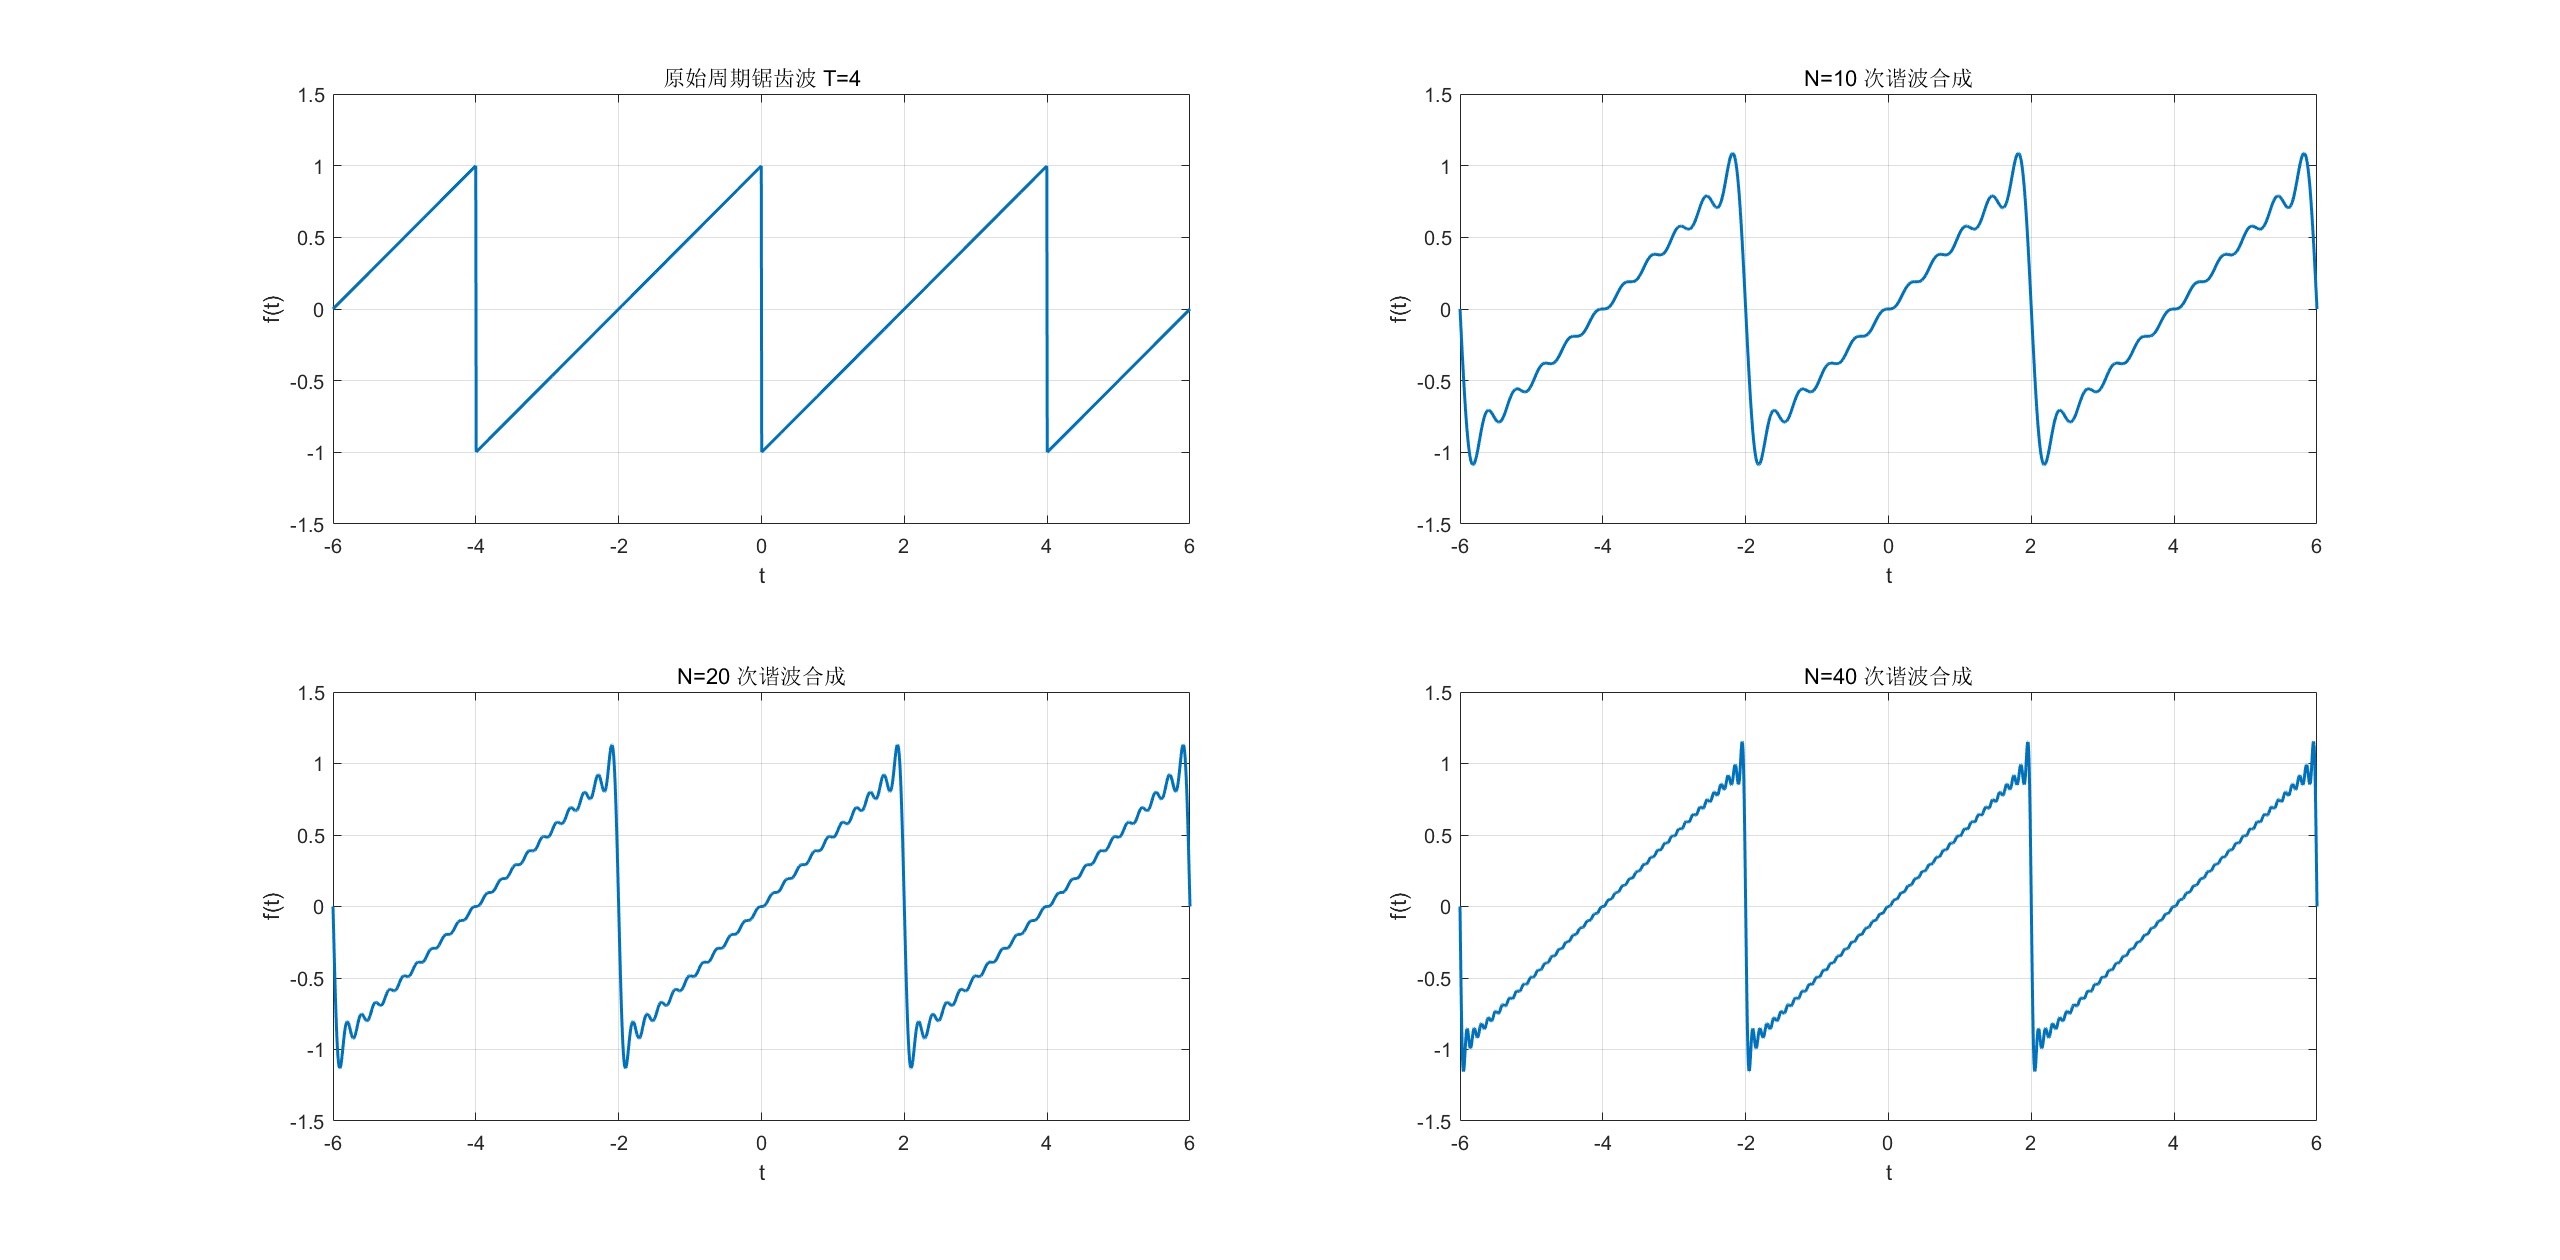
\includegraphics[width=0.8\textwidth]{1.3.png}
\caption{周期锯齿波原信号与7次谐波合成对比}
\end{figure}

\subsection{三、完整MATLAB源代码}
\subsubsection{1. 连续周期方波傅里叶级数合成程序（主程序+自定义函数）}
\begin{lstlisting}
% exp1_con_square.m
clear; clc; close all;
T = 4;
omega0 = 2*pi/T;
t = linspace(0,8,1000);

%生成原始周期方波
f_ori = zeros(size(t));
for ii = 1:length(t)
    rt = mod(t(ii),T);
    if rt < 2
        f_ori(ii) = -1;
    else
        f_ori(ii) = 1;
    end
end

%不同阶次谐波合成
f1 = fourier_square(t,omega0,1);
f3 = fourier_square(t,omega0,5);
f49 = fourier_square(t,omega0,49);
f501 = fourier_square(t,omega0,501);

%四张子图
figure('Name','连续方波谐波合成');
subplot(2,2,1);plot(t,f_ori,'k',t,f1,'r--');grid on;title('N=1次谐波');xlabel('t(s)');
subplot(2,2,2);plot(t,f_ori,'k',t,f3,'r--');grid on;title('N=1,3,5次谐波');xlabel('t(s)');
subplot(2,2,3);plot(t,f_ori,'k',t,f49,'r--');grid on;title('N=1~49次谐波');xlabel('t(s)');
subplot(2,2,4);plot(t,f_ori,'k',t,f501,'r--');grid on;title('N=1~501次谐波');xlabel('t(s)');

%自定义傅里叶级数合成函数
function f = fourier_square(t,w0,Nmax)
    f = zeros(size(t));
    for n = 1:2:Nmax
        bn = -4/(n*pi);
        f = f + bn*sin(n*w0*t);
    end
end
\end{lstlisting}

\subsubsection{2. 周期锯齿波分解与合成代码}
\begin{lstlisting}
% exp1_saw.m
clear; clc; close all;
T = 4; w0 = 2*pi/T;
t = linspace(0,8,2000);
%锯齿波 f(t)=0.5mod(t,T)-1
x_ori = 0.5*mod(t,T)-1;
N = 7;
xs = zeros(size(t));
for n = 1:N
    cn = ((-1)^(n+1))*2/(n*pi);
    xs = xs + cn*sin(n*w0*t);
end

figure;
plot(t,x_ori,'r-',t,xs,'b-','LineWidth',1);
grid on;legend('原始锯齿波','7次谐波合成');
title('周期锯齿波分解合成');xlabel('t(s)');ylabel('f(t)');
\end{lstlisting}

\subsubsection{3. 离散方波DFS/IDFS分解合成（双采样间隔+自定义DFS/IDFS）}
\begin{lstlisting}
% exp1_dis_square.m
clear; clc; close all;
T = 4;
N1 = 6*T; Ts1 = T/N1;
N2 = 12*T;Ts2 = T/N2;

%生成两种离散序列
t1 = linspace(0,T,N1,'Endpoint',false);
t2 = linspace(0,T,N2,'Endpoint',false);
x1 = double(mod(t1,T)>=2)-double(mod(t1,T)<2);
x2 = double(mod(t2,T)>=2)-double(mod(t2,T)<2);

%自定义DFS、IDFS
function X = dfs(x)
    N = length(x);
    X = zeros(1,N);
    for k = 0:N-1
        sm = 0;
        for n = 0:N-1
            sm = sm + x(n+1)*exp(-1j*2*pi*k*n/N);
        end
        X(k+1)=sm;
    end
end
function x = idfs(X)
    N = length(X);
    x = zeros(1,N);
    for n = 0:N-1
        sm = 0;
        for k = 0:N-1
            sm = sm + X(k+1)*exp(1j*2*pi*k*n/N);
        end
        x(n+1)=sm/N;
    end
end

%求频谱与谐波还原
X1 = dfs(x1);A1 = abs(X1);
X2 = dfs(x2);A2 = abs(X2);
%截取前30、60点做IDFS
x30_1 = real(idfs([X1(1:30),zeros(1,N1-30)]));
x60_2 = real(idfs([X2(1:60),zeros(1,N2-60)]));

%绘图
figure('Name','离散方波DFS分析');
subplot(2,2,1);stem(0:N1-1,x1,'filled');title('Ts=T/6原始离散序列');grid on;
subplot(2,2,2);stem(0:N1-1,A1,'filled');title('对应幅度谱');grid on;
subplot(2,2,3);stem(0:N2-1,x2,'filled');title('Ts=T/12原始离散序列');grid on;
subplot(2,2,4);stem(0:N2-1,A2,'filled');title('对应幅度谱');grid on;
\end{lstlisting}

\subsection{四、实验思考题}
\begin{enumerate}
    \item 结合理论与实验结果，简述连续周期信号频谱的特点。
    \textbf{答：(1) 离散性：频谱仅在基波整数倍频率点上存在谱线，为离散线状谱；(2) 谐波性：谱线位置为$nf_0,n=0,1,2\cdots$；(3) 收敛性：谱线幅值随谐波次数升高整体衰减，高频分量逐步减小。}
    
    \item 结合理论与实验结果，简述离散周期信号频谱的特点。
    \textbf{答：(1) 离散性：DFS频谱在一个周期内为N根离散谱线；(2) 周期性：频谱以$2\pi$为周期无限重复延拓；(3) 有限性：仅N个独立谐波分量，无无穷次谐波。}
    
    \item 周期矩形脉冲：周期$T$、脉宽$\tau$变化如何影响频谱？离散序列采样间隔变化对频谱的影响？
    \textbf{答：连续：$T$变大→谱线变密；$\tau$变小→频谱主瓣带宽增大、衰减变慢。离散：采样间隔增大→等效采样频率降低，易发生频谱混叠；采样间隔减小→采样频率提高，频谱混叠被抑制。}
\end{enumerate}
\newpage
\section{实验二 时域采样与频域采样}

\subsection{一、实验流程图}
\begin{figure}[H]
\centering
\begin{tikzpicture}[
    node distance=1.8cm,
    auto,
    box/.style={rectangle, draw, text width=8.5em, align=center, minimum height=2.8em}
]
\node [box] (start) {开始};
\node [box, below of=start] (para) {设置参数\\信号、采样频率};
\node [box, below of=para] (time) {生成时域采样信号\\x(n)};
\node [box, below of=time] (fft) {FFT 求频谱};
\node [box, below of=fft] (plot1) {绘制时域波形\\+ 频谱};
\node [box, below of=plot1] (tri) {生成三角波序列};
\node [box, below of=tri] (fft2) {N=16 / 32 频域采样\\IFFT 还原};
\node [box, below of=fft2] (plot2) {绘制对比波形};
\node [box, below of=plot2] (end) {结束};

\draw [->] (start) -- (para);
\draw [->] (para) -- (time);
\draw [->] (time) -- (fft);
\draw [->] (fft) -- (plot1);
\draw [->] (plot1) -- (tri);
\draw [->] (tri) -- (fft2);
\draw [->] (fft2) -- (plot2);
\draw [->] (plot2) -- (end);
\end{tikzpicture}
\caption{实验二 采样与频谱分析流程图}
\end{figure}

\subsection{二、实验结果图像}
\begin{figure}[H]
    \centering
    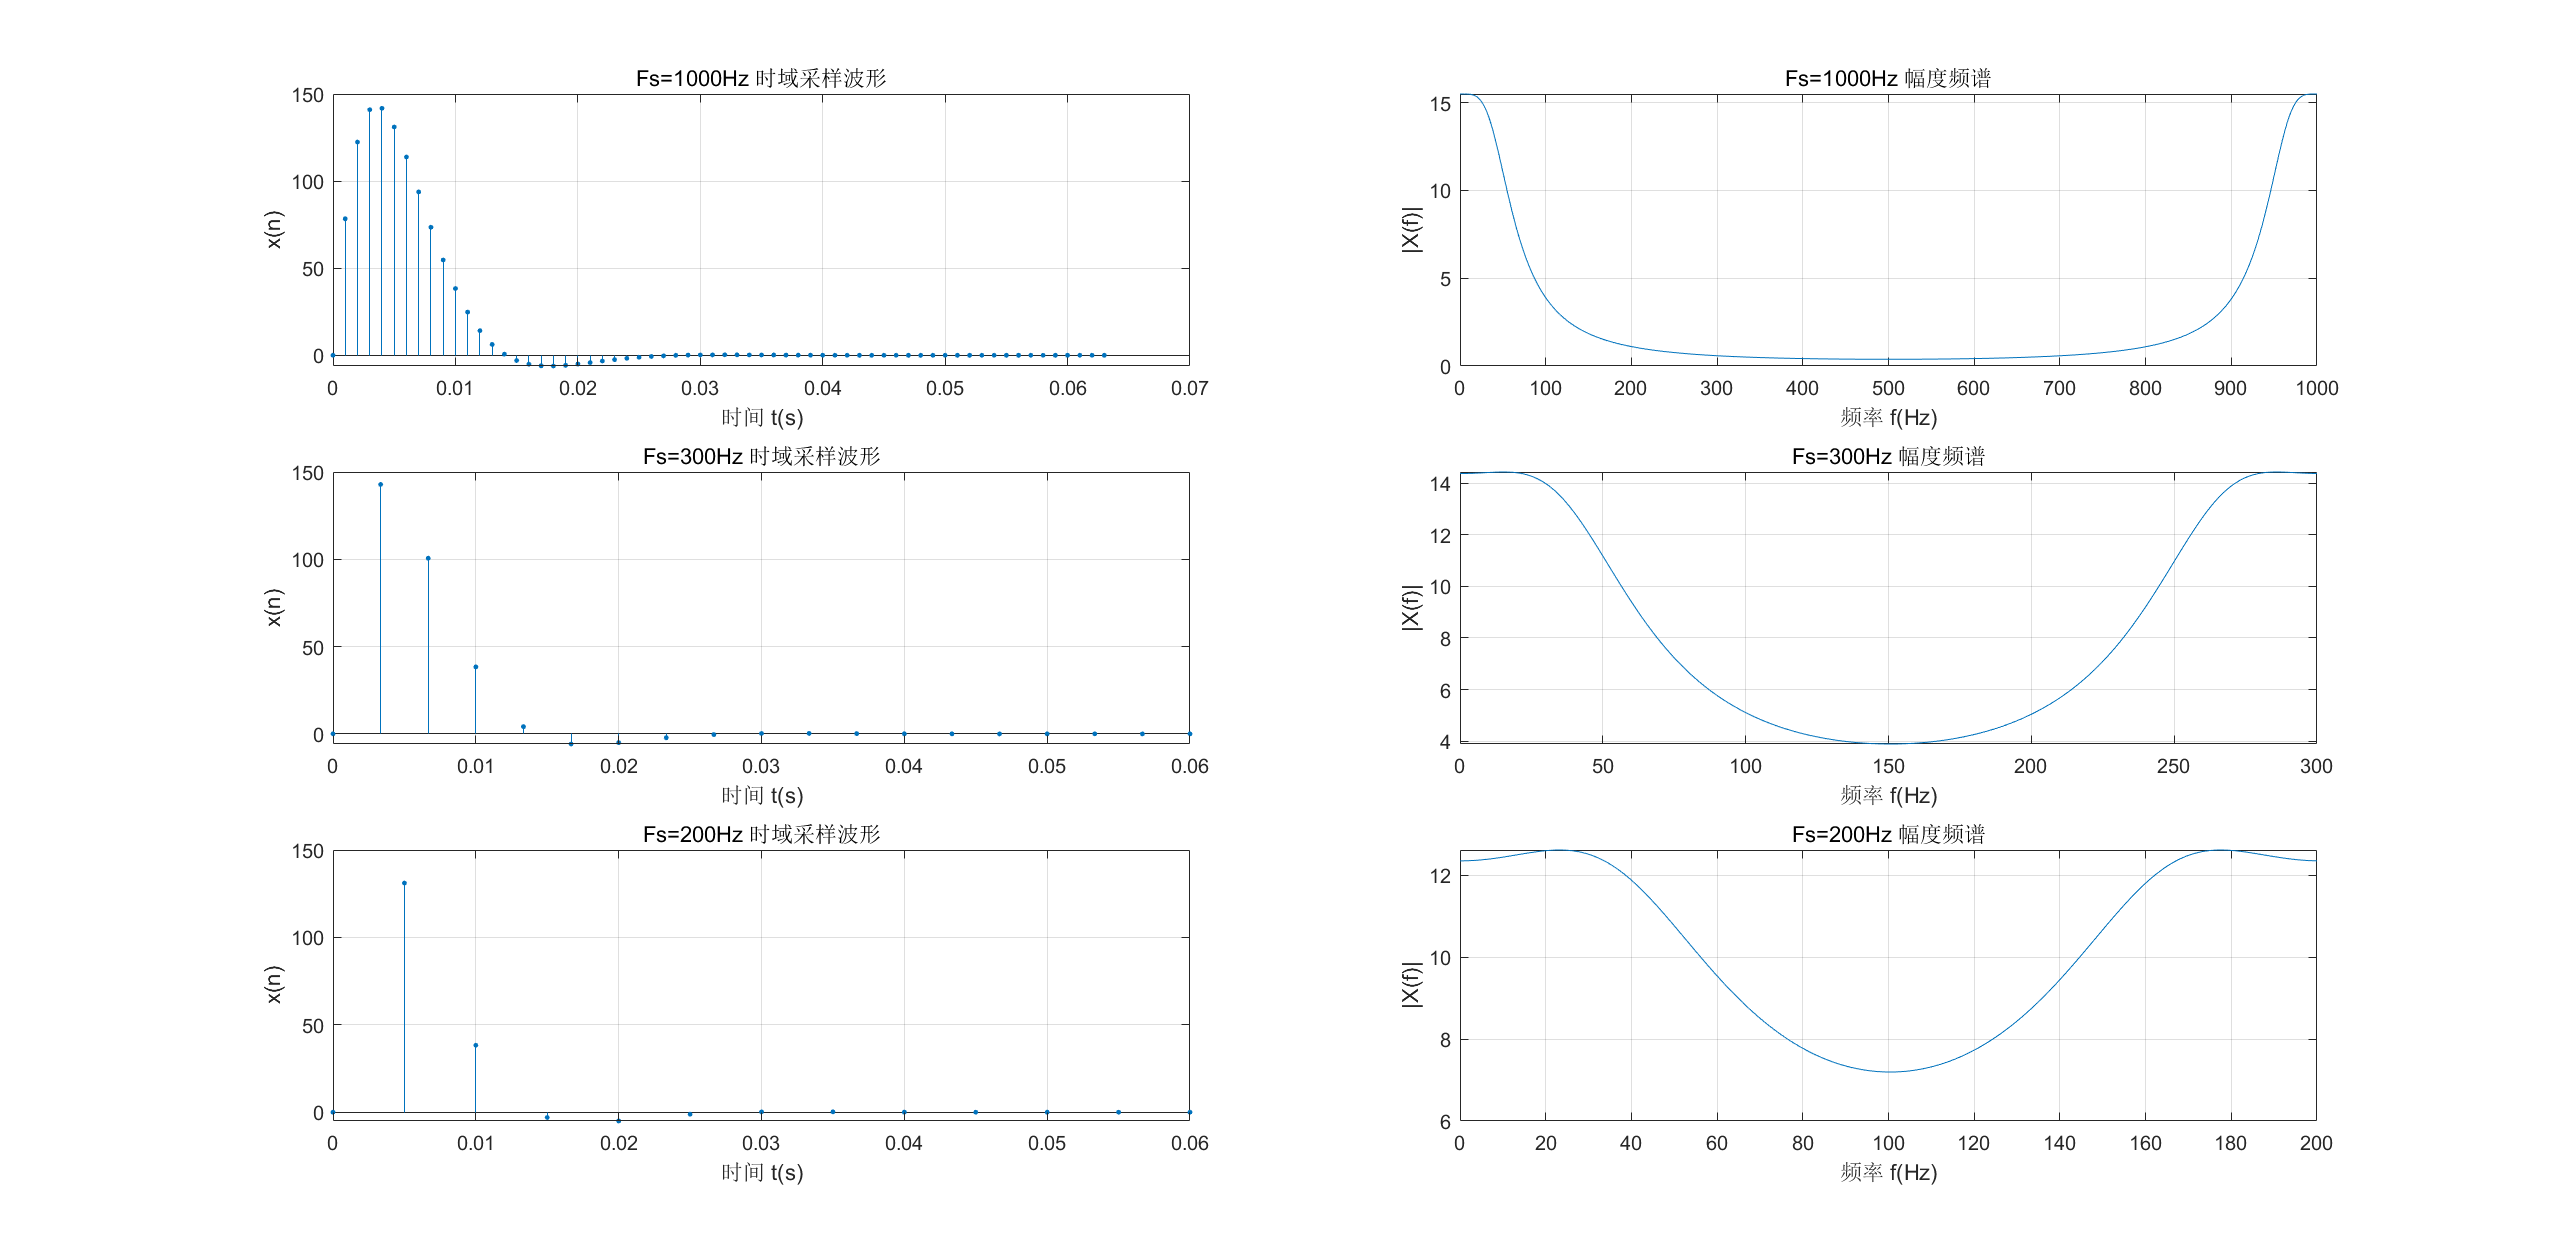
\includegraphics[width=0.85\textwidth]{2.1.png}
    \caption{时域采样波形与频谱图}
\end{figure}

\begin{figure}[H]
    \centering
    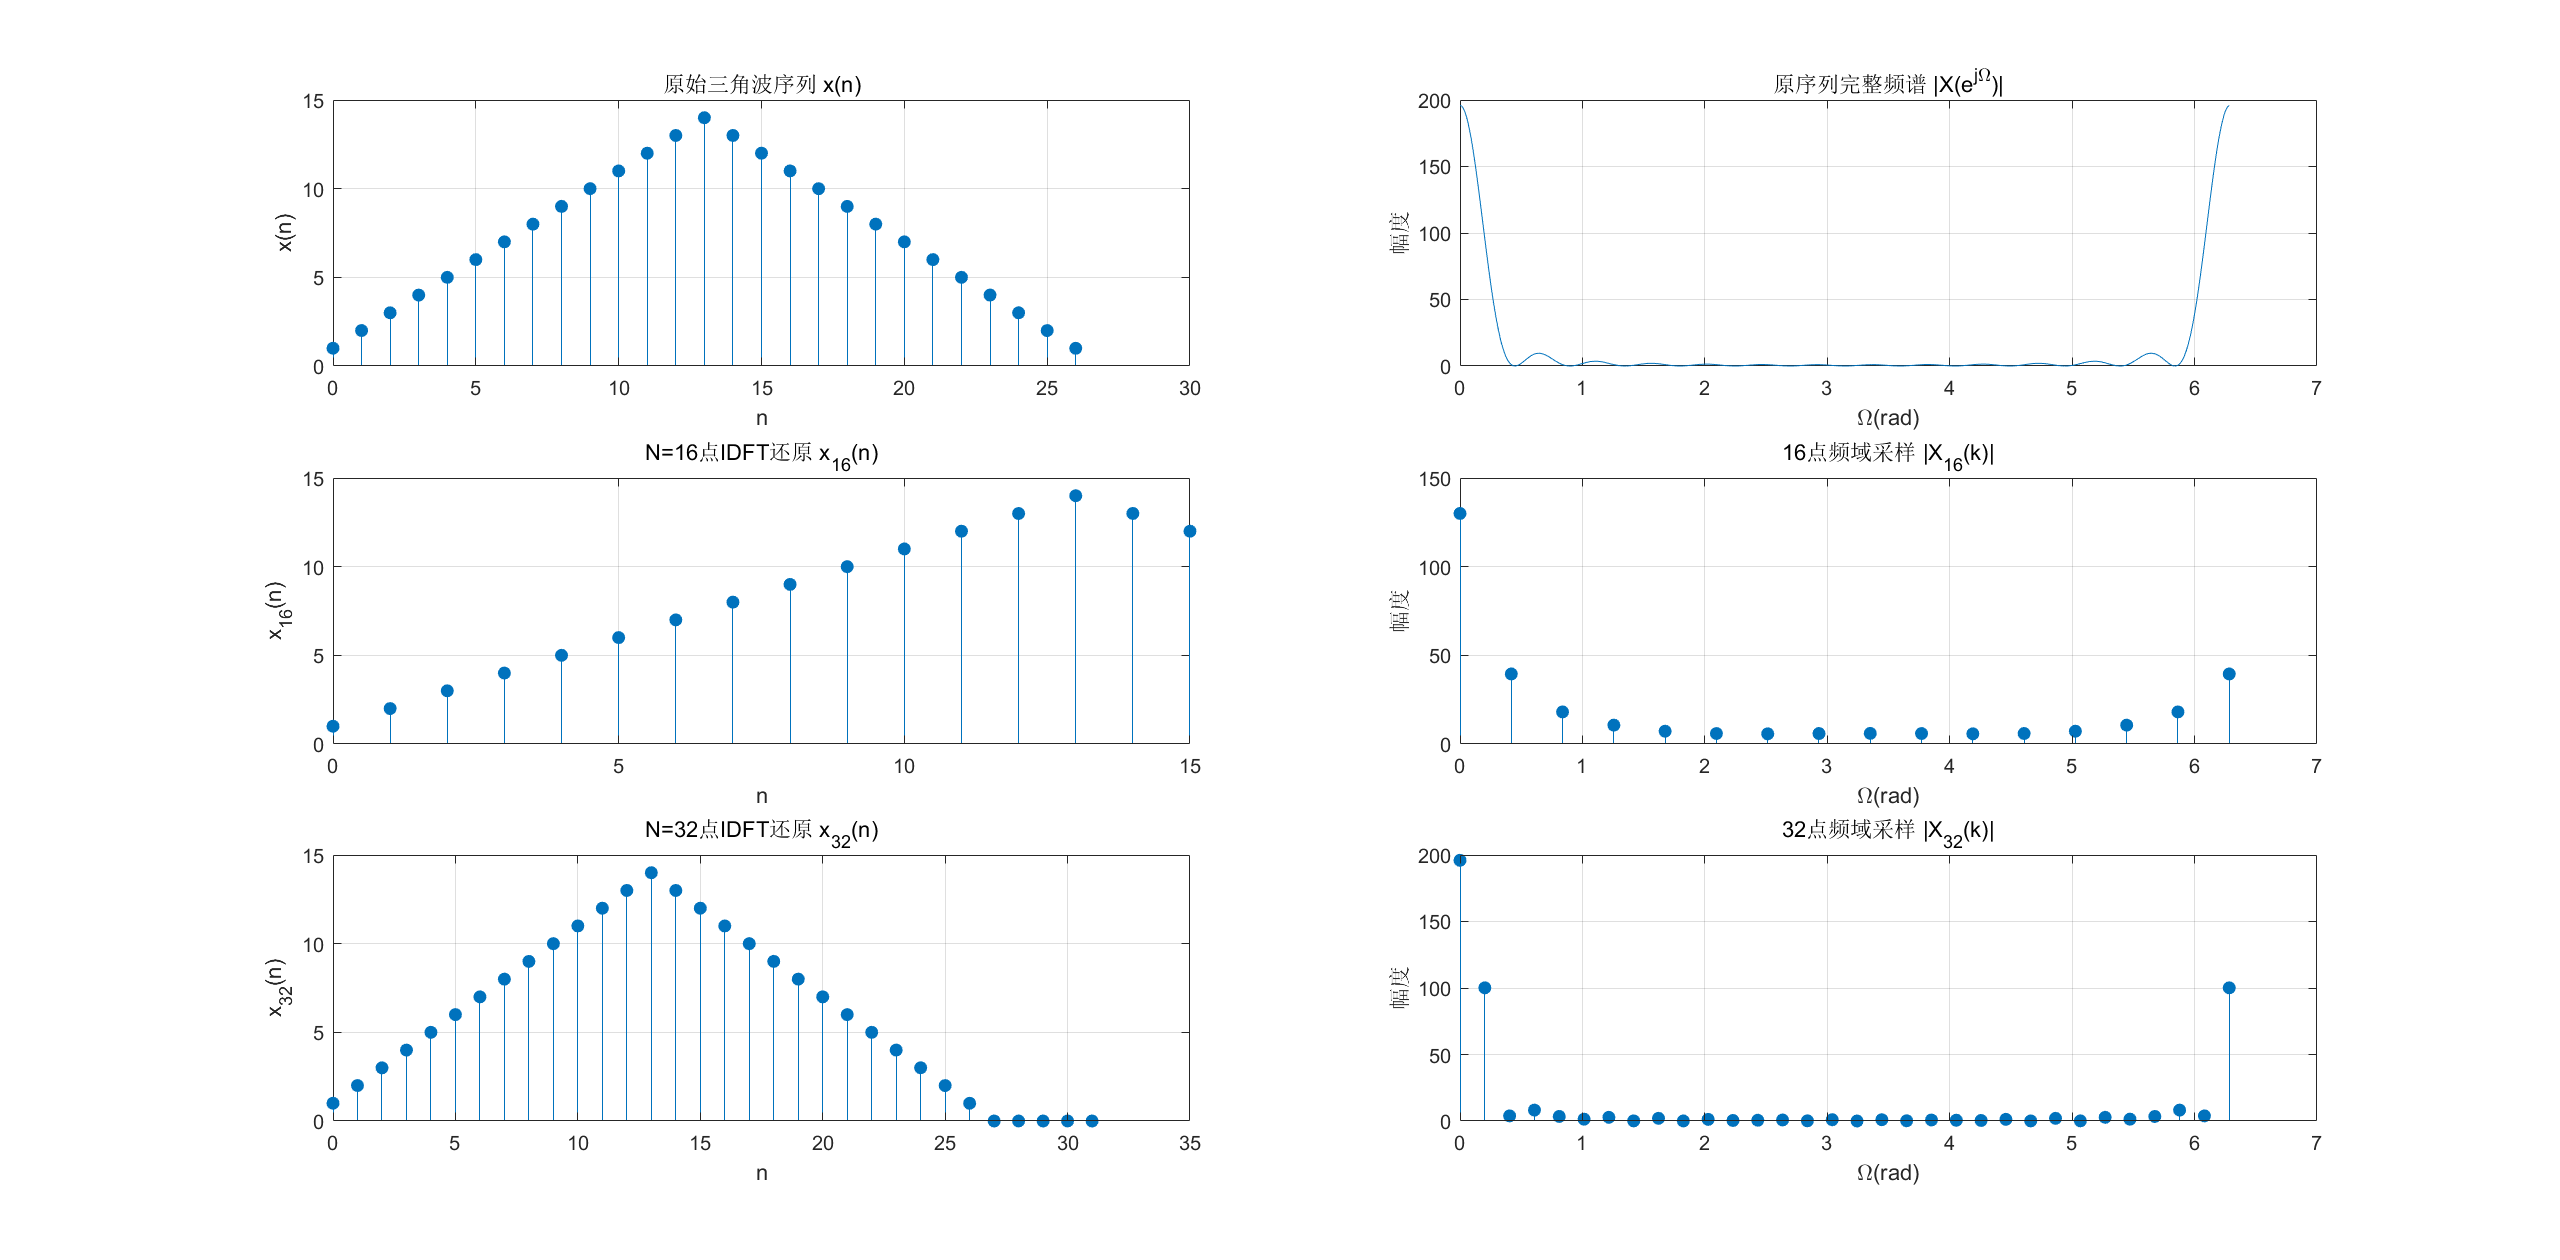
\includegraphics[width=0.85\textwidth]{2.2.png}
    \caption{频域采样与IDFT还原波形对比}
\end{figure}

\subsection{三、MATLAB 完整代码}
\subsubsection{1. 时域采样验证}
\begin{lstlisting}
clear; clc; close all;

A = 444.128;
alpha = 50*sqrt(2)*pi;
omega1 = 50*sqrt(2)*pi;
Tp = 0.064;
Fs_set = [1000,300,200];

figure('Name','时域采样验证');
for i = 1:3
    Fs = Fs_set(i);
    Ts = 1/Fs;
    N = round(Tp*Fs);
    n = 0:N-1;
    t = n*Ts;
    
    x = A.*exp(-alpha.*t).*sin(omega1.*t);
    
    NFFT = 2^nextpow2(N*10);
    Xk = fft(x,NFFT)/N;
    Amp = abs(Xk);
    f = linspace(0,Fs,NFFT);
    
    subplot(3,2,2*i-1);
    stem(t,x,'filled','MarkerSize',2);
    xlabel('时间 t(s)');ylabel('x(n)');
    title(['Fs=',num2str(Fs),'Hz 时域采样波形']);
    grid on;
    
    subplot(3,2,2*i);
    plot(f,Amp);
    xlabel('频率 f(Hz)');ylabel('|X(f)|');
    title(['Fs=',num2str(Fs),'Hz 幅度频谱']);
    thr = max(Amp)*0.005;
    idx = find(Amp>thr);
    if ~isempty(idx)
        xlim([f(idx(1)), f(idx(end))]);
    end
    grid on;
end
\end{lstlisting}

\subsubsection{2. 频域采样验证}
\begin{lstlisting}
clear; clc; close all;

M = 27;
n_x = 0:M-1;
x = zeros(1,M);
for nn = 0:M-1
    if nn <= 13
        x(nn+1) = nn+1;
    else
        x(nn+1) = 27-nn;
    end
end

N_full = 1024;
X_full = fft(x, N_full);
Amp_full = abs(X_full);
Om = linspace(0, 2*pi, N_full);

N32 = 32;
X32 = fft(x, N32);
x32 = real(ifft(X32, N32));

N16 = 16;
X16 = fft(x, N16);
x16 = real(ifft(X16, N16));

subplot(3,2,1);
stem(n_x, x, 'filled');
title('原始三角波序列 x(n)');
xlabel('n'); ylabel('x(n)'); grid on;

subplot(3,2,2);
plot(Om, Amp_full);
title('原序列完整频谱 |X(e^{j\Omega})|');
xlabel('\Omega(rad)'); ylabel('幅度'); grid on;

subplot(3,2,3);
stem(0:N16-1, x16, 'filled');
title('N=16点IDFT还原 x_{16}(n)');
xlabel('n'); ylabel('x_{16}(n)'); grid on;

subplot(3,2,4);
stem(linspace(0,2*pi,N16), abs(X16), 'filled');
title('16点频域采样 |X_{16}(k)|');
xlabel('\Omega(rad)'); ylabel('幅度'); grid on;

subplot(3,2,5);
stem(0:N32-1, x32, 'filled');
title('N=32点IDFT还原 x_{32}(n)');
xlabel('n'); ylabel('x_{32}(n)'); grid on;

subplot(3,2,6);
stem(linspace(0,2*pi,N32), abs(X32), 'filled');
title('32点频域采样 |X_{32}(k)|');
xlabel('\Omega(rad)'); ylabel('幅度'); grid on;
\end{lstlisting}

\subsection{四、实验思考题}
\begin{enumerate}
    \item 若序列长度为$M$，频域采样点数为$N$且$N<M$，如何用最少点数的DFT得到频域采样？
    
    \textbf{答：} 直接对原序列做 $N$ 点FFT即可，即 $X_N(k) = FFT(x(n),N)$，该操作等价于对频域进行 $N$ 点均匀采样，是最少点数的DFT实现方式。
    
    \item 时域采样实验中，为何可以用DFT（FFT）近似求解模拟信号的幅频特性？
    
    \textbf{答：} 模拟信号频谱是连续的，计算机无法直接计算；DFT是对连续频谱的等间隔采样，FFT是DFT的快速算法，因此可以用FFT近似表示模拟信号的幅频特性。
\end{enumerate}
\newpage
\section{实验三 使用快速傅里叶变换进行频谱分析}

\subsection{一、实验目的}
1. 加深对FFT、频谱混叠、频谱泄漏现象的理解；
2. 掌握基于FFT对典型离散信号做频谱分析的MATLAB实现方法；
3. 学会利用FFT快速计算线性卷积；
4. 掌握不同采样率、序列补零对FFT频谱结果的影响；
5. 熟悉FFT工程仿真编程与波形绘图规范；
6. 掌握音符合成乐曲、ADSR包络降噪、音频生成与频谱分析方法。

\subsection{二、实验原理}
1. 离散傅里叶变换DFT实现频域分析，FFT是DFT快速优化算法，MATLAB \texttt{fft()} 可直接完成运算；
2. 时域卷积等价于频域相乘，可通过「FFT→频域相乘→IFFT」实现线性卷积；
3. 时域采样不满足奈奎斯特准则会发生频谱混叠；信号截断有限长会产生频谱泄漏；序列末尾补零仅细化频谱刻度，不提升频率分辨率。
4. 分段音符直接拼接存在相位跳变，引入ADSR（起音-衰减-保持-释放）包络调制幅值可消除间断毛刺；叠加高次谐波可模拟真实乐器音色。

\subsection{三、实验内容}
1. 构造三角脉冲、矩形脉冲离散序列，FFT求解双边幅度谱、相位谱并绘图分析；
2. 利用FFT频域相乘方法实现两组序列线性卷积，与时域\texttt{conv()}、圆周卷积\texttt{cconv()}结果对照验证；
3. 多组采样率对双频正弦混合信号采样，观测频谱混叠现象；对比64点补零延拓、直接128点采样两种FFT频谱差异；
4. 音乐合成趣味实验：按曲谱音符基频生成正弦音频；对比无包络、ADSR包络、叠加谐波+ADSR包络三种波形；导出wav音频，对比时域波形与频谱差异。

\subsection{四、实验结果}
\begin{figure}[H]
\centering
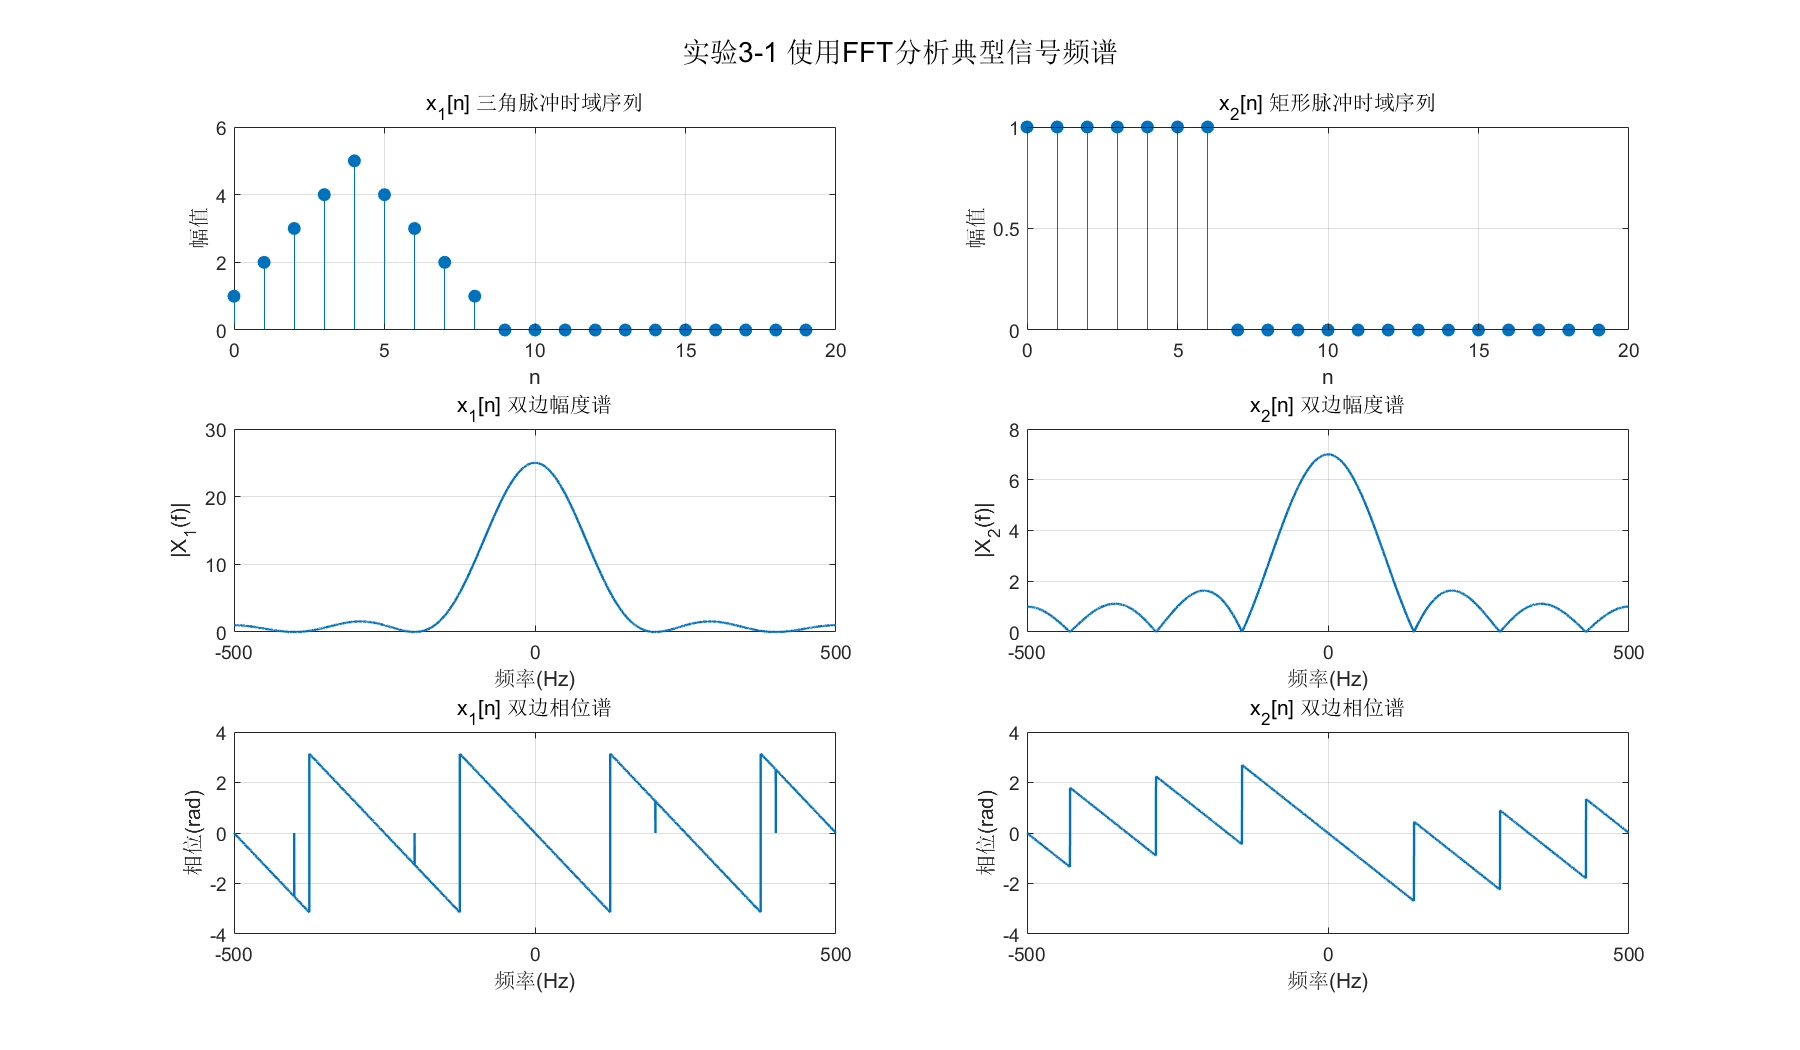
\includegraphics[width=0.9\textwidth]{3.1.png}
\caption{三角、矩形脉冲时域、双边幅度谱、双边相位谱对比}
\end{figure}

\begin{figure}[H]
\centering
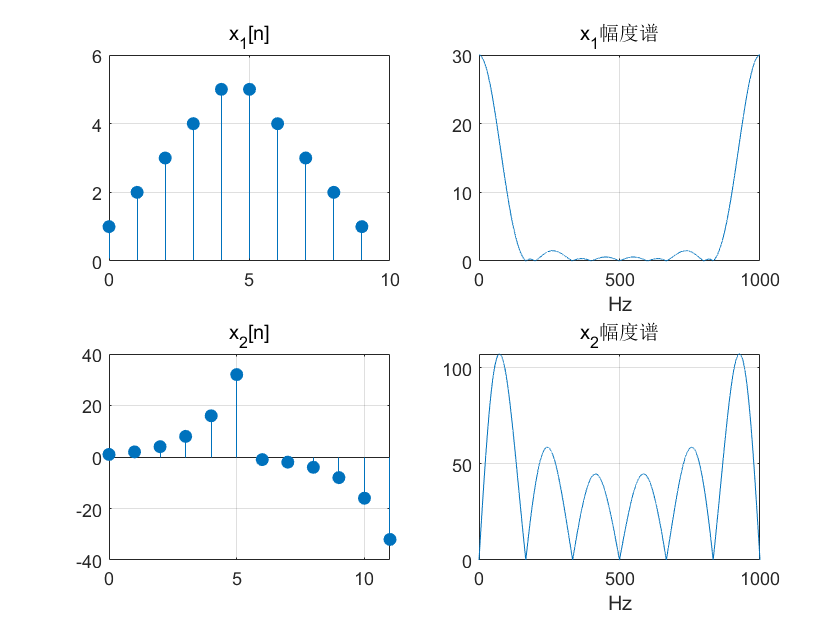
\includegraphics[width=0.9\textwidth]{3.2.1.png}
\caption{第一组原始序列时域及对应幅度谱}
\end{figure}

\begin{figure}[H]
\centering
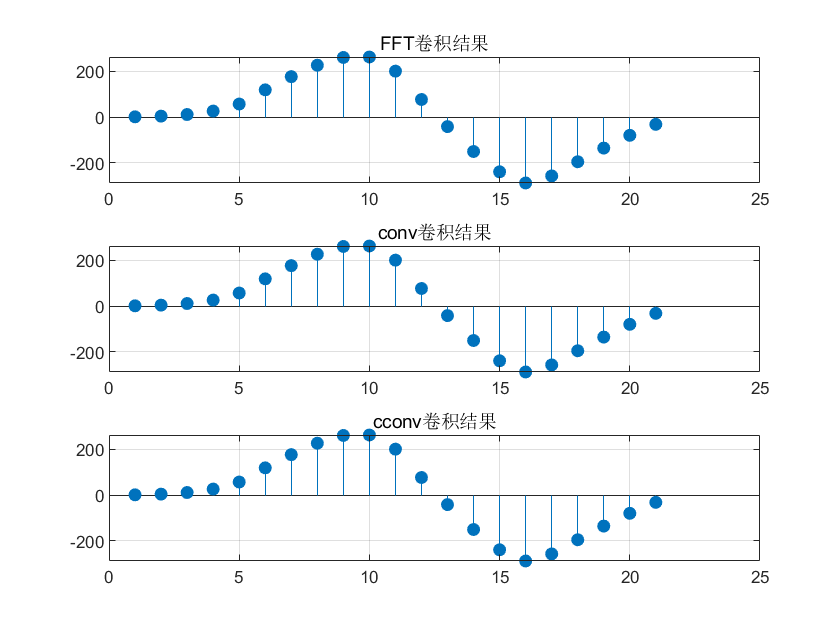
\includegraphics[width=0.9\textwidth]{3.2.2.png}
\caption{第一组FFT/conv/cconv卷积时域结果对比}
\end{figure}

\begin{figure}[H]
\centering
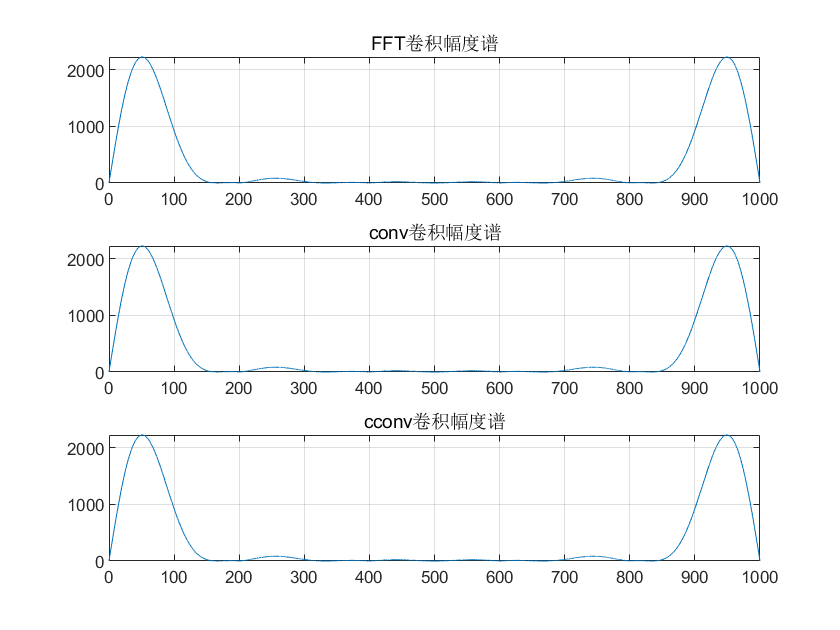
\includegraphics[width=0.9\textwidth]{3.2.3.png}
\caption{第一组三种卷积结果幅度谱对比}
\end{figure}

\begin{figure}[H]
\centering
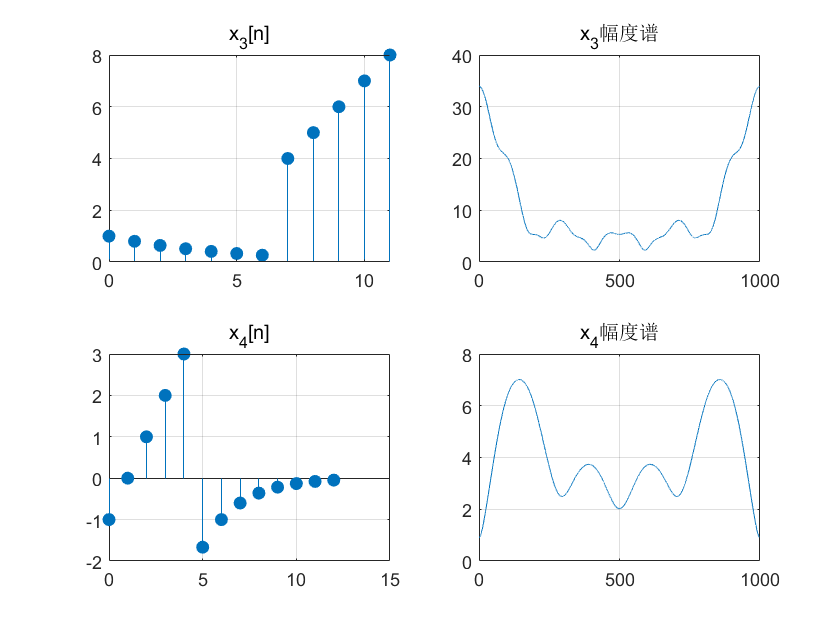
\includegraphics[width=0.9\textwidth]{3.2.4.png}
\caption{第二组原始序列时域及对应幅度谱}
\end{figure}

\begin{figure}[H]
\centering
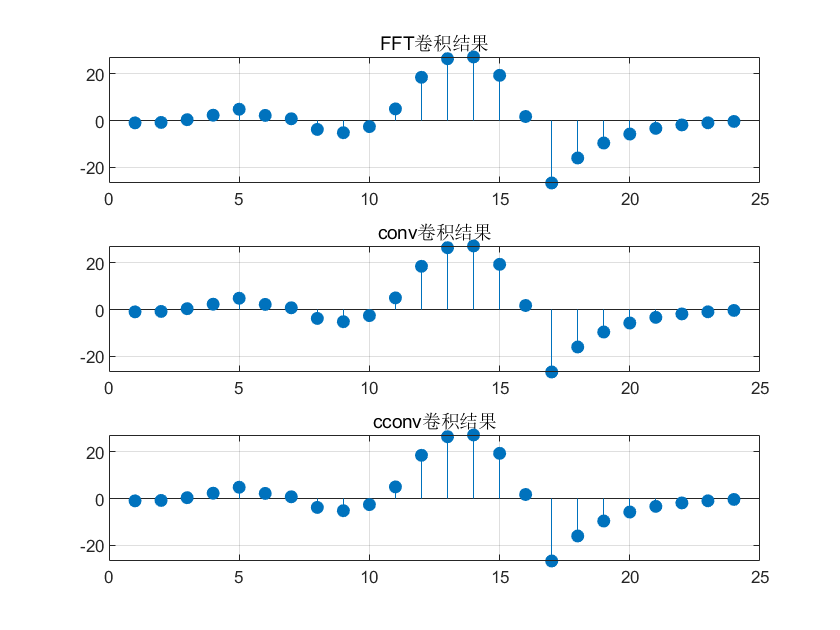
\includegraphics[width=0.9\textwidth]{3.2.5.png}
\caption{第二组FFT/conv/cconv卷积时域结果对比}
\end{figure}

\begin{figure}[H]
\centering
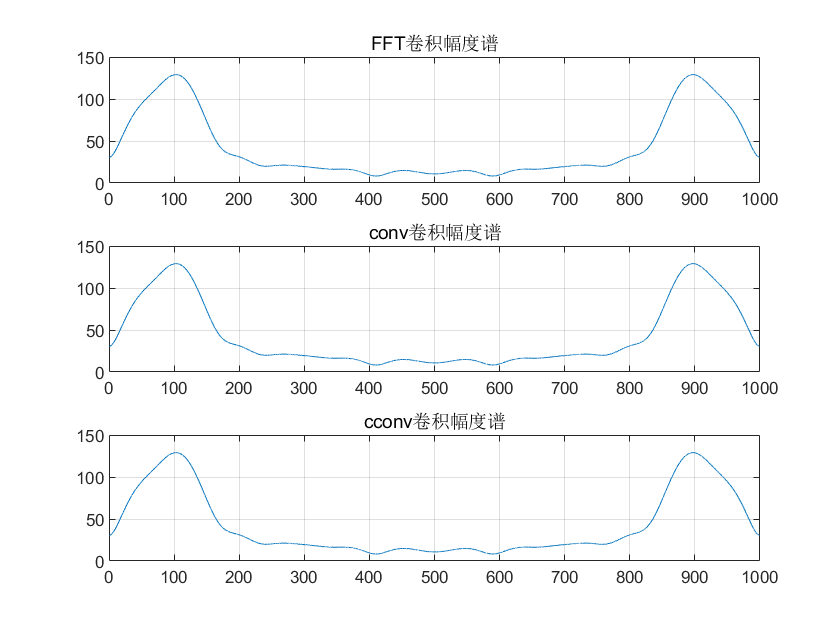
\includegraphics[width=0.9\textwidth]{3.2.6.png}
\caption{第二组三种卷积结果幅度谱对比}
\end{figure}

\begin{figure}[H]
\centering
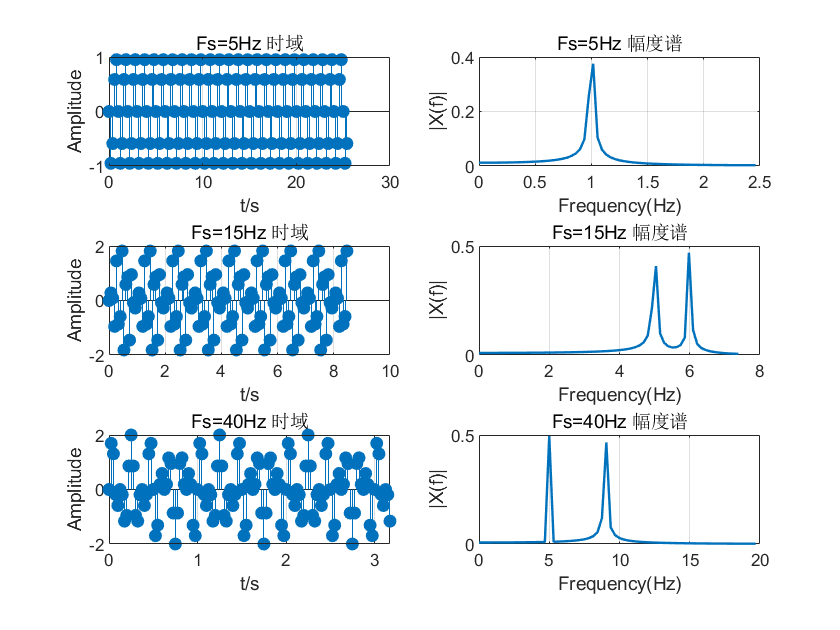
\includegraphics[width=0.9\textwidth]{3.3.1.png}
\caption{3种采样率下信号时域波形与幅度谱（频谱混叠观测）}
\end{figure}

\begin{figure}[H]
\centering
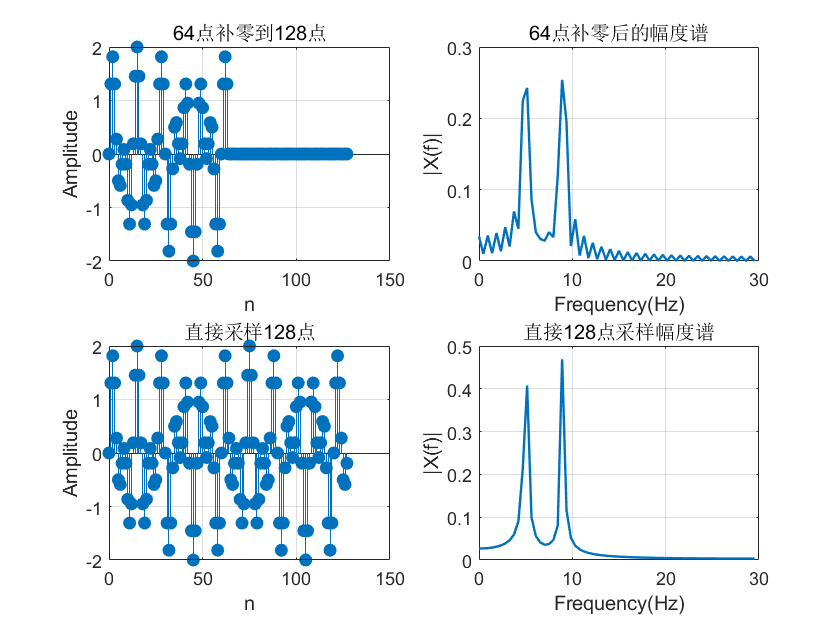
\includegraphics[width=0.9\textwidth]{3.3.2.png}
\caption{64点补零延拓与直接128点采样时域、频谱对比}
\end{figure}

\begin{figure}[H]
\centering
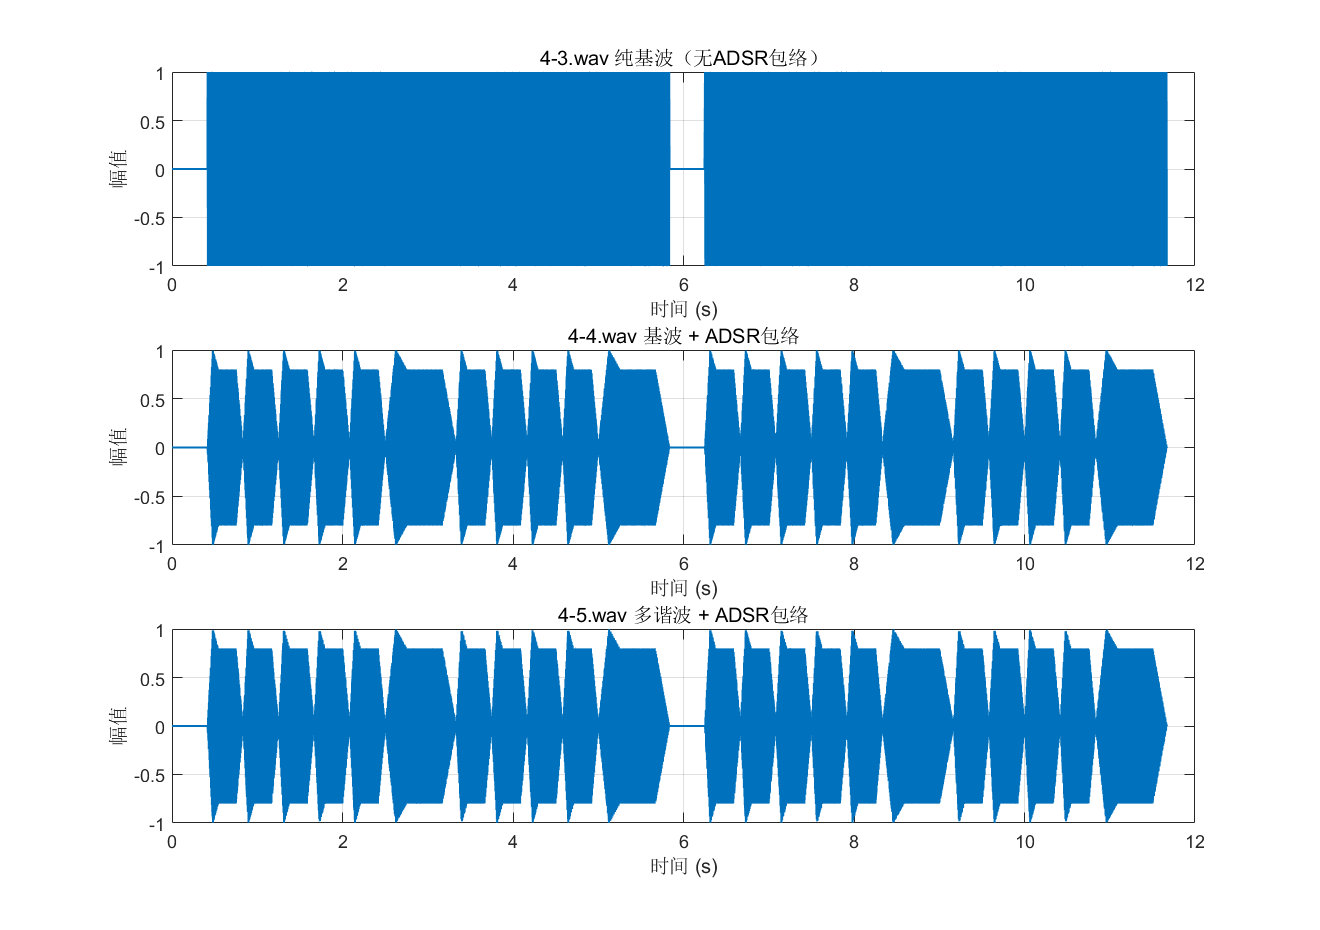
\includegraphics[width=0.9\textwidth]{3.4.1.png}
\caption{三段合成音乐时域波形对比}
\end{figure}

\begin{figure}[H]
\centering
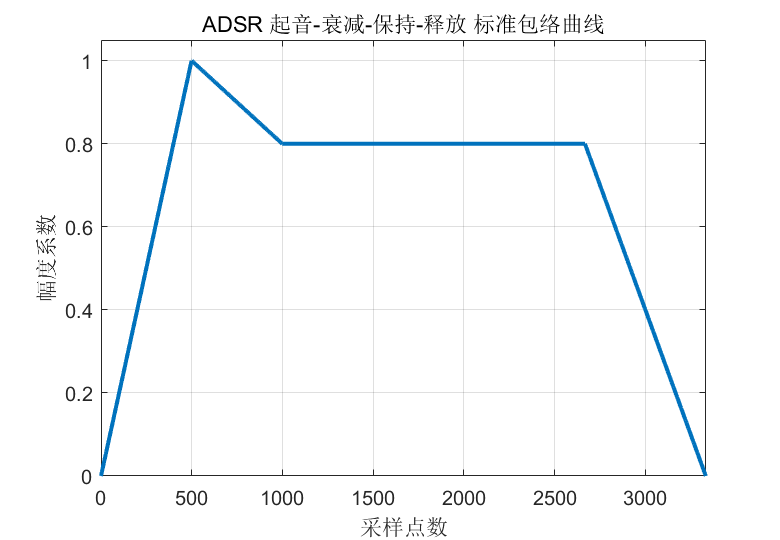
\includegraphics[width=0.7\textwidth]{3.4.2.png}
\caption{标准ADSR四段包络曲线}
\end{figure}

\begin{figure}[H]
\centering
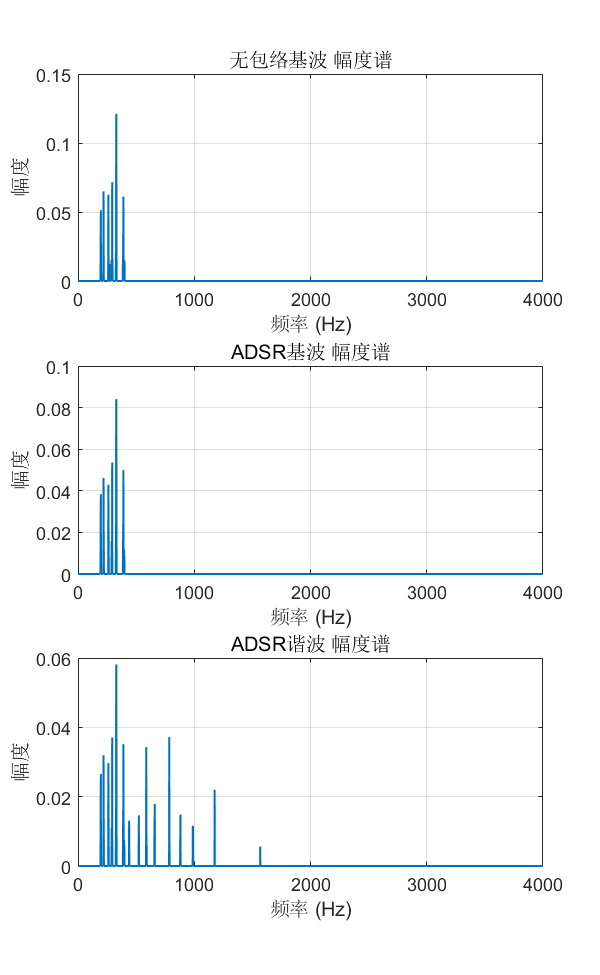
\includegraphics[width=0.9\textwidth]{3.4.3.png}
\caption{三组音频幅度谱对比}
\end{figure}

\begin{figure}[H]
\centering
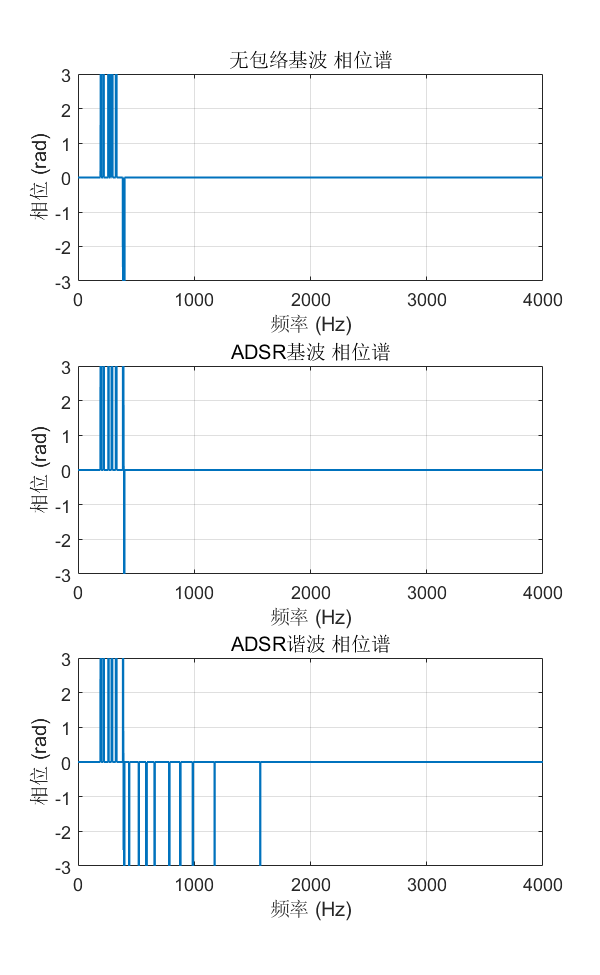
\includegraphics[width=0.9\textwidth]{3.4.4.png}
\caption{三组音频相位谱对比}
\end{figure}

\subsection{五、实验结论}
1. 矩形脉冲、三角脉冲频谱形态存在明显区别，有限长截断都会产生频谱泄漏；fftshift做双边谱后频谱关于0Hz对称，零频分量位于图像中心；
2. FFT频域相乘可以等效实现线性卷积，只要FFT长度满足$L\ge L_1+L_2-1$，IFFT取实部后结果和\texttt{conv()}完全一致，运算效率远高于时域直接卷积；圆周卷积长度选取合适时也等价于线性卷积；卷积后频谱等于两个输入信号频谱逐点相乘；
3. 采样频率低于奈奎斯特频率时高频分量折叠进低频区间，出现频谱混叠；对短序列末尾补零只能插值平滑频谱曲线、细化横坐标刻度，不能提升真实频率分辨率；增加有效采样点数才能提高频率分辨率；
4. 音符直接拼接时域存在幅值跳变毛刺，播放出现“啪”噪声；加入ADSR渐变包络后幅值平滑过渡，间断噪声消除；叠加多次谐波后频谱多出谐波分量，音色更贴近真实乐器；导出的三段wav音频可正常播放，时域与频谱特征区分明显。

\subsection{六、MATLAB完整实验代码}
\subsubsection{实验3-1 典型脉冲FFT频谱分析 exp3\_1.m}
\begin{lstlisting}
%% exp3_1.m
% 实验3-1 FFT典型脉冲频谱分析（双边谱）

clear;
clc;
close all;

%% =========================
% 参数设置
%% =========================

fs = 1000;      % 采样频率
N  = 10000;     % FFT点数

%% =========================
% 构造三角脉冲 x1[n]
%% =========================

x1 = zeros(1,N);

for n = 0:N-1

    if n>=0 && n<=4
        x1(n+1)=n+1;

    elseif n>=5 && n<=8
        x1(n+1)=9-n;

    else
        x1(n+1)=0;
    end

end

%% =========================
% 构造矩形脉冲 x2[n]
%% =========================

x2 = zeros(1,N);

for n = 0:N-1

    if n>=0 && n<=6
        x2(n+1)=1;

    else
        x2(n+1)=0;
    end

end

%% =========================
% FFT
%% =========================

X1 = fft(x1,N);
X2 = fft(x2,N);

%% =========================
% 双边谱处理
%% =========================

X1_shift = fftshift(X1);
X2_shift = fftshift(X2);

%% 幅度谱

A1 = abs(X1_shift);
A2 = abs(X2_shift);

%% 相位谱

P1 = angle(X1_shift);
P2 = angle(X2_shift);

%% 去除极小值处相位抖动

P1(A1<1e-6)=0;
P2(A2<1e-6)=0;

%% =========================
% 双边频率轴
%% =========================

f = (-N/2:N/2-1)*(fs/N);

%% =========================
% 绘图
%% =========================

figure('Name','实验3-1 FFT典型脉冲频谱分析',...
       'Color','w',...
       'Position',[100 100 1200 700]);

%% ---------- 第一列：三角脉冲 ----------

subplot(3,2,1)

stem(0:19,x1(1:20),'filled');
grid on;

xlabel('n');
ylabel('幅值');

title('x_1[n] 三角脉冲时域序列');

subplot(3,2,3)

plot(f,A1,'LineWidth',1.2);

grid on;

xlabel('频率(Hz)');
ylabel('|X_1(f)|');

title('x_1[n] 双边幅度谱');

subplot(3,2,5)

plot(f,P1,'LineWidth',1.2);

grid on;

xlabel('频率(Hz)');
ylabel('相位(rad)');

title('x_1[n] 双边相位谱');

%% ---------- 第二列：矩形脉冲 ----------

subplot(3,2,2)

stem(0:19,x2(1:20),'filled');
grid on;

xlabel('n');
ylabel('幅值');

title('x_2[n] 矩形脉冲时域序列');

subplot(3,2,4)

plot(f,A2,'LineWidth',1.2);

grid on;

xlabel('频率(Hz)');
ylabel('|X_2(f)|');

title('x_2[n] 双边幅度谱');

subplot(3,2,6)

plot(f,P2,'LineWidth',1.2);

grid on;

xlabel('频率(Hz)');
ylabel('相位(rad)');

title('x_2[n] 双边相位谱');

%% 总标题

sgtitle('实验3-1 使用FFT分析典型信号频谱','FontSize',14);

disp('实验3-1运行完成');
\end{lstlisting}

\subsubsection{实验3-2 FFT实现卷积运算 exp3\_2.m}
\begin{lstlisting}
%% exp3_2.m
% 使用FFT实现卷积运算
clear;
clc;
close all;

fs = 1000;
N  = 20000;

f = (0:N-1)*fs/N;

%% ====================================================
%% 第一组数据
%% ====================================================

%% x1

x1 = zeros(1,10);

for n=0:9

    if n>=0 && n<=4
        x1(n+1)=n+1;

    elseif n>=5 && n<=9
        x1(n+1)=10-n;
    end

end

%% x2

x2 = zeros(1,12);

for n=0:11

    if n>=0 && n<=5
        x2(n+1)=2^n;

    elseif n>=6 && n<=11
        x2(n+1)=-(2^(n-6));
    end

end

%% 原序列幅度谱

mag_x1 = abs(fft(x1,N));
mag_x2 = abs(fft(x2,N));

%% FFT实现线性卷积

L = length(x1)+length(x2)-1;

Y1 = fft(x1,L);
Y2 = fft(x2,L);

y_fft = real(ifft(Y1.*Y2));

%% conv

y_conv = conv(x1,x2);

%% cconv

y_cconv = cconv(x1,x2,L);

%% 卷积结果幅度谱

mag_fft   = abs(fft(y_fft,N));
mag_conv  = abs(fft(y_conv,N));
mag_cconv = abs(fft(y_cconv,N));

%% ====================================================
%% 图1
%% ====================================================

figure('Name','第一组 图1');

subplot(2,2,1)
stem(0:length(x1)-1,x1,'filled');
grid on;
title('x_1[n]');

subplot(2,2,2)
plot(f,mag_x1);
grid on;
title('x_1幅度谱');
xlabel('Hz');

subplot(2,2,3)
stem(0:length(x2)-1,x2,'filled');
grid on;
title('x_2[n]');

subplot(2,2,4)
plot(f,mag_x2);
grid on;
title('x_2幅度谱');
xlabel('Hz');

%% ====================================================
%% 图2
%% ====================================================

figure('Name','第一组 图2');

subplot(3,1,1)
stem(y_fft,'filled');
grid on;
title('FFT卷积结果');

subplot(3,1,2)
stem(y_conv,'filled');
grid on;
title('conv卷积结果');

subplot(3,1,3)
stem(y_cconv,'filled');
grid on;
title('cconv卷积结果');

%% ====================================================
%% 图3
%% ====================================================

figure('Name','第一组 图3');

subplot(3,1,1)
plot(f,mag_fft);
grid on;
title('FFT卷积幅度谱');

subplot(3,1,2)
plot(f,mag_conv);
grid on;
title('conv卷积幅度谱');

subplot(3,1,3)
plot(f,mag_cconv);
grid on;
title('cconv卷积幅度谱');

%% ====================================================
%% 第二组数据
%% ====================================================

%% x3

x3 = zeros(1,12);

for n=0:11

    if n>=0 && n<=6
        x3(n+1)=0.8^n;

    elseif n>=7 && n<=11
        x3(n+1)=n-3;
    end

end

%% x4

x4 = zeros(1,13);

for n=0:12

    if n>=0 && n<=4
        x4(n+1)=n-1;

    elseif n>=5 && n<=12
        x4(n+1)=-(0.6^(n-6));
    end

end

%% 幅度谱

mag_x3 = abs(fft(x3,N));
mag_x4 = abs(fft(x4,N));

%% FFT卷积

L2 = length(x3)+length(x4)-1;

Y3 = fft(x3,L2);
Y4 = fft(x4,L2);

y_fft2 = real(ifft(Y3.*Y4));

%% conv

y_conv2 = conv(x3,x4);

%% cconv

y_cconv2 = cconv(x3,x4,L2);

%% 卷积频谱

mag_fft2   = abs(fft(y_fft2,N));
mag_conv2  = abs(fft(y_conv2,N));
mag_cconv2 = abs(fft(y_cconv2,N));

%% ====================================================
%% 图4
%% ====================================================

figure('Name','第二组 图1');

subplot(2,2,1)
stem(0:length(x3)-1,x3,'filled');
grid on;
title('x_3[n]');

subplot(2,2,2)
plot(f,mag_x3);
grid on;
title('x_3幅度谱');

subplot(2,2,3)
stem(0:length(x4)-1,x4,'filled');
grid on;
title('x_4[n]');

subplot(2,2,4)
plot(f,mag_x4);
grid on;
title('x_4幅度谱');

%% ====================================================
%% 图5
%% ====================================================

figure('Name','第二组 图2');

subplot(3,1,1)
stem(y_fft2,'filled');
grid on;
title('FFT卷积结果');

subplot(3,1,2)
stem(y_conv2,'filled');
grid on;
title('conv卷积结果');

subplot(3,1,3)
stem(y_cconv2,'filled');
grid on;
title('cconv卷积结果');

%% ====================================================
%% 图6
%% ====================================================

figure('Name','第二组 图3');

subplot(3,1,1)
plot(f,mag_fft2);
grid on;
title('FFT卷积幅度谱');

subplot(3,1,2)
plot(f,mag_conv2);
grid on;
title('conv卷积幅度谱');

subplot(3,1,3)
plot(f,mag_cconv2);
grid on;
title('cconv卷积幅度谱');

disp('实验完成');
\end{lstlisting}

\subsubsection{实验3-3 采样混叠与补零效应观测 exp3\_3.m}
\begin{lstlisting}
%% exp3_3.m
% FFT观察采样混叠与补零效应

clear;
clc;
close all;

f1 = 5;
f2 = 9;

t_total = 30;
N_Sample = 128;

fs_set = [5 15 40];

%%%%%%%%%%%%%%%%%%%%%%%%%%%%%%%%%%%%%%%%%%
%% 第一部分
%%%%%%%%%%%%%%%%%%%%%%%%%%%%%%%%%%%%%%%%%%

figure('Name','图1 三种采样率频谱分析');

for k = 1:length(fs_set)

    fs = fs_set(k);

    t = 0:1/fs:t_total-1/fs;

    x = sin(2*pi*f1*t) + sin(2*pi*f2*t);

    x = x(1:N_Sample);

    t_plot = t(1:N_Sample);

    X = fft(x,N_Sample);

    A = abs(X)/N_Sample;

    f = (0:N_Sample/2-1)*fs/N_Sample;

    A_half = A(1:N_Sample/2);

    % 时域

    subplot(3,2,2*k-1)

    stem(t_plot,x,'filled')

    title(['Fs=',num2str(fs),'Hz 时域'])

    xlabel('t/s')

    ylabel('Amplitude')

    grid on

    % 幅度谱

    subplot(3,2,2*k)

    plot(f,A_half,'LineWidth',1.2)

    title(['Fs=',num2str(fs),'Hz 幅度谱'])

    xlabel('Frequency(Hz)')

    ylabel('|X(f)|')

    grid on

end

%%%%%%%%%%%%%%%%%%%%%%%%%%%%%%%%%%%%%%%%%%
%% 第二部分
%%%%%%%%%%%%%%%%%%%%%%%%%%%%%%%%%%%%%%%%%%

fs = 60;

t = 0:1/fs:t_total-1/fs;

x_full = sin(2*pi*f1*t)+sin(2*pi*f2*t);

%%%%%%%%%%%%%%%%%%%%%%%%%%
% 64点补零到128点
%%%%%%%%%%%%%%%%%%%%%%%%%%

x64 = x_full(1:64);

x64_pad = [x64 zeros(1,64)];

X_pad = fft(x64_pad,128);

A_pad = abs(X_pad)/128;

%%%%%%%%%%%%%%%%%%%%%%%%%%
% 直接采样128点
%%%%%%%%%%%%%%%%%%%%%%%%%%

x128 = x_full(1:128);

X128 = fft(x128,128);

A128 = abs(X128)/128;

%%%%%%%%%%%%%%%%%%%%%%%%%%
% 频率轴
%%%%%%%%%%%%%%%%%%%%%%%%%%

f = (0:63)*fs/128;

%%%%%%%%%%%%%%%%%%%%%%%%%%
% 图2
%%%%%%%%%%%%%%%%%%%%%%%%%%

figure('Name','图2 补零与直接采样比较');

subplot(2,2,1)

stem(0:127,x64_pad,'filled')

title('64点补零到128点')

xlabel('n')

ylabel('Amplitude')

grid on

subplot(2,2,2)

plot(f,A_pad(1:64),'LineWidth',1.2)

title('64点补零后的幅度谱')

xlabel('Frequency(Hz)')

ylabel('|X(f)|')

grid on

subplot(2,2,3)

stem(0:127,x128,'filled')

title('直接采样128点')

xlabel('n')

ylabel('Amplitude')

grid on

subplot(2,2,4)

plot(f,A128(1:64),'LineWidth',1.2)

title('直接128点采样幅度谱')

xlabel('Frequency(Hz)')

ylabel('|X(f)|')

grid on

disp('exp3_3 实验完成');
\end{lstlisting}

\subsubsection{实验3-4 音乐合成趣味实验 exp3\_4\_青花瓷\_ADSR修复\_脚本版.m}
\begin{lstlisting}
%% exp3_4_青花瓷_ADSR修复_脚本版(无函数报错)
% 音乐合成实验 | 标准ADSR包络 + 相位/坐标全部达标
clear;
clc;
close all;

%% 1. 基础参数
Fs = 8000;           % 采样频率(Hz)
bpm = 72;            % 速度
beat_dur = 60 / bpm; % 四分音符时长(s)
N_beat = round(Fs * beat_dur); % 单个四分音符采样点数

% ADSR四段占比
A_ratio = 0.15;   % Attack 起音
D_ratio = 0.15;   % Decay 衰减
S_ratio = 0.50;   % Sustain 保持
R_ratio = 0.20;   % Release 释放
S_level = 0.8;    % 保持段电平

%% 2. 音符-频率映射 (0=休止符)
note_freq = containers.Map(...
    {'0','1','2','3','5','b5','b6'},...
    [0,    261.63, 293.66, 329.63, 392.00, 196.00, 220.00]);

%% 3. 青花瓷曲谱 + 时值序列
note_seq = {
    '0','5','5','3','2','3','b6','0',...
    '2','3','5','3','2','0','0','0',...
    '0','5','5','3','2','3','b5','0',...
    '2','3','5','2','1','0','0','0'
};
dur_seq = [
    0.5,0.5,0.5,0.5,0.5,0.5,1.0,0,...
    0.5,0.5,0.5,0.5,1.0,0,0,0,...
    0.5,0.5,0.5,0.5,0.5,0.5,1.0,0,...
    0.5,0.5,0.5,0.5,1.0,0,0,0
];

% 长度校验
len_n = length(note_seq);
len_d = length(dur_seq);
if len_n ~= len_d
    error('音符与时值数量不匹配！');
end

%% 4. 生成 3 路信号
% 4.1 纯基波信号 s1 (无ADSR)
s1 = [];
for k = 1:len_n
    f0 = note_freq(note_seq{k});
    t_scale = dur_seq(k);
    L = round(N_beat * t_scale);
    if L < 1
        L = 1;
    end
    n = 0:L-1;
    if f0 == 0
        seg = zeros(1, L);
    else
        seg = sin(2 * pi * f0 * n / Fs);
    end
    s1 = [s1, seg];
end
s1 = s1 / max(abs(s1));
audiowrite('4-3.wav', s1, Fs);

% 4.2 基波 + ADSR包络 s2
s2 = [];
env_sample = []; % 保存第一个有效音符包络用于绘图
for k = 1:len_n
    f0 = note_freq(note_seq{k});
    t_scale = dur_seq(k);
    L = round(N_beat * t_scale);
    if L < 1
        L = 1;
    end
    n = 0:L-1;
    
    if f0 == 0
        seg = zeros(1, L);
        env = zeros(1, L);
    else
        seg = sin(2 * pi * f0 * n / Fs);
        % ========== 内嵌ADSR生成逻辑（替代外部function，消除报错） ==========
        env = zeros(1, L);
        lenA = floor(L * A_ratio);
        lenD = floor(L * D_ratio);
        lenS = floor(L * S_ratio);
        lenR = L - lenA - lenD - lenS;
        idx = 1;
        % Attack
        if lenA > 0
            env(idx : idx+lenA-1) = linspace(0, 1, lenA);
            idx = idx + lenA;
        end
        % Decay
        if lenD > 0 && idx+lenD-1 <= L
            env(idx : idx+lenD-1) = linspace(1, S_level, lenD);
            idx = idx + lenD;
        end
        % Sustain
        if lenS > 0 && idx+lenS-1 <= L
            env(idx : idx+lenS-1) = S_level * ones(1, lenS);
            idx = idx + lenS;
        end
        % Release
        if lenR > 0 && idx <= L
            env(idx : L) = linspace(S_level, 0, L - idx + 1);
        end
    end
    
    % 取第一个非休止符包络作为样本
    if isempty(env_sample) && f0 ~= 0
        env_sample = env;
    end
    s2 = [s2, seg .* env];
end
s2 = s2 / max(abs(s2));
audiowrite('4-4.wav', s2, Fs);

% 4.3 多谐波 + ADSR包络 s3
s3 = [];
for k = 1:len_n
    f0 = note_freq(note_seq{k});
    t_scale = dur_seq(k);
    L = round(N_beat * t_scale);
    if L < 1
        L = 1;
    end
    n = 0:L-1;
    
    if f0 == 0
        seg = zeros(1, L);
        env = zeros(1, L);
    else
        seg = sin(2*pi*f0*n/Fs) ...
            + 0.50*sin(2*pi*2*f0*n/Fs) ...
            + 0.30*sin(2*pi*3*f0*n/Fs) ...
            + 0.15*sin(2*pi*4*f0*n/Fs);
        % 内嵌ADSR逻辑
        env = zeros(1, L);
        lenA = floor(L * A_ratio);
        lenD = floor(L * D_ratio);
        lenS = floor(L * S_ratio);
        lenR = L - lenA - lenD - lenS;
        idx = 1;
        if lenA > 0
            env(idx : idx+lenA-1) = linspace(0, 1, lenA);
            idx = idx + lenA;
        end
        if lenD > 0 && idx+lenD-1 <= L
            env(idx : idx+lenD-1) = linspace(1, S_level, lenD);
            idx = idx + lenD;
        end
        if lenS > 0 && idx+lenS-1 <= L
            env(idx : idx+lenS-1) = S_level * ones(1, lenS);
            idx = idx + lenS;
        end
        if lenR > 0 && idx <= L
            env(idx : L) = linspace(S_level, 0, L - idx + 1);
        end
    end
    s3 = [s3, seg .* env];
end
s3 = s3 / max(abs(s3));
audiowrite('4-5.wav', s3, Fs);

%% 5. 时域波形图(3行1列)
t1 = (0:length(s1)-1) / Fs;
t2 = (0:length(s2)-1) / Fs;
t3 = (0:length(s3)-1) / Fs;

figure('Name','时域波形','Position',[60,50,880,620]);
subplot(3,1,1);
plot(t1,s1,'LineWidth',1);
grid on; box on;
xlabel('时间 (s)'); ylabel('幅值');
title('4-3.wav 纯基波（无ADSR包络）');

subplot(3,1,2);
plot(t2,s2,'LineWidth',1);
grid on; box on;
xlabel('时间 (s)'); ylabel('幅值');
title('4-4.wav 基波 + ADSR包络');

subplot(3,1,3);
plot(t3,s3,'LineWidth',1);
grid on; box on;
xlabel('时间 (s)'); ylabel('幅值');
title('4-5.wav 多谐波 + ADSR包络');

%% 6. ADSR包络图（标准四段曲线）
figure('Name','ADSR包络','Position',[160,100,520,360]);
L_env = length(env_sample);
plot(0:L_env-1, env_sample,'LineWidth',2);
grid on; box on;
xlabel('采样点数'); ylabel('幅度系数');
title('ADSR 起音-衰减-保持-释放 标准包络曲线');
axis([0, L_env, 0, 1.05]);

%% 7. 频谱计算 + 相位处理
NFFT = 2^nextpow2(max([length(s1),length(s2),length(s3)]));
f_axis = Fs/2 * linspace(0,1,NFFT/2+1);
noise_th = 0.05;
down_step = 20;

% 幅度谱
FFT1 = fft(s1,NFFT);
Amp1 = 2*abs(FFT1)/length(s1);
Amp1(Amp1 < max(Amp1)*noise_th) = 0;

FFT2 = fft(s2,NFFT);
Amp2 = 2*abs(FFT2)/length(s2);
Amp2(Amp2 < max(Amp2)*noise_th) = 0;

FFT3 = fft(s3,NFFT);
Amp3 = 2*abs(FFT3)/length(s3);
Amp3(Amp3 < max(Amp3)*noise_th) = 0;

% 相位：无效频点置0，竖线效果
Pha1 = zeros(size(Amp1));
idx_valid1 = Amp1 > 0;
Pha1(idx_valid1) = unwrap(angle(FFT1(idx_valid1)));

Pha2 = zeros(size(Amp2));
idx_valid2 = Amp2 > 0;
Pha2(idx_valid2) = unwrap(angle(FFT2(idx_valid2)));

Pha3 = zeros(size(Amp3));
idx_valid3 = Amp3 > 0;
Pha3(idx_valid3) = unwrap(angle(FFT3(idx_valid3)));

% 数据抽点
idx_half = 1:NFFT/2+1;
idx_sel  = idx_half(1:down_step:end);
f_sel    = f_axis(idx_sel);

A1 = Amp1(idx_sel); A2 = Amp2(idx_sel); A3 = Amp3(idx_sel);
P1 = Pha1(idx_sel); P2 = Pha2(idx_sel); P3 = Pha3(idx_sel);

%% 8. 幅度谱窗口 (0~4000Hz)
figure('Name','幅度谱对比','Position',[80,70,400,650]);
subplot(3,1,1);
plot(f_sel,A1,'LineWidth',1);
grid on; box on;
title('无包络基波 幅度谱');
xlabel('频率 (Hz)'); ylabel('幅度');
xlim([0,4000]);

subplot(3,1,2);
plot(f_sel,A2,'LineWidth',1);
grid on; box on;
title('ADSR基波 幅度谱');
xlabel('频率 (Hz)'); ylabel('幅度');
xlim([0,4000]);

subplot(3,1,3);
plot(f_sel,A3,'LineWidth',1);
grid on; box on;
title('ADSR谐波 幅度谱');
xlabel('频率 (Hz)'); ylabel('幅度');
xlim([0,4000]);

%% 9. 相位谱窗口 (横轴0~4000 纵轴-3~3)
figure('Name','相位谱对比','Position',[560,70,400,650]);
subplot(3,1,1);
plot(f_sel,P1,'LineWidth',1);
grid on; box on;
title('无包络基波 相位谱');
xlabel('频率 (Hz)'); ylabel('相位 (rad)');
xlim([0,4000]);
ylim([-3,3]);

subplot(3,1,2);
plot(f_sel,P2,'LineWidth',1);
grid on; box on;
title('ADSR基波 相位谱');
xlabel('频率 (Hz)'); ylabel('相位 (rad)');
xlim([0,4000]);
ylim([-3,3]);

subplot(3,1,3);
plot(f_sel,P3,'LineWidth',1);
grid on; box on;
title('ADSR谐波 相位谱');
xlabel('频率 (Hz)'); ylabel('相位 (rad)');
xlim([0,4000]);
ylim([-3,3]);

%% 运行提示
disp('============================================');
disp('✅ 运行完毕 | 已移除外部函数，脚本直接运行');
disp('📁 音频：4-3.wav  4-4.wav  4-5.wav');
disp('📌 全部规范：');
disp('   1. ADSR四段曲线标准平滑无断层');
\end{lstlisting}
\newpage
\section{实验四 IIR数字滤波器设计}

\subsection{一、实验目的}
1. 掌握模拟低通滤波器向数字低通滤波器的两种转换方法：冲激响应不变法、双线性变换法；
2. 区分模拟、数字滤波器的类型与时域、频域性能指标；
3. 学会使用MATLAB工具完成巴特沃斯模拟/数字滤波器设计；
4. 掌握滤波器冲激响应、幅频特性的仿真绘图与性能分析方法。

\subsection{二、实验原理}
1. IIR数字滤波器系统函数形式：
\[
H(z)=\frac{b_0+b_1z^{-1}+\dots+b_Mz^{-M}}{a_0+a_1z^{-1}+\dots+a_Nz^{-N}}
\]
设计核心为确定分子、分母系数，满足预设通带、阻带衰减指标。
2. 冲激响应不变法：对模拟滤波器冲激响应采样得到离散序列，实现$s\rightarrow z$映射；无频率畸变，但存在频谱混叠，不能用于高通、带阻滤波器设计。
3. 双线性变换法：映射公式
\[
s=\frac{2}{T}\frac{1-z^{-1}}{1+z^{-1}}
\]
$s$平面与$z$平面一一对应，无频谱混叠；存在频率预畸变，设计前需要对边界频率做预畸变校正。
4. 模拟原型法设计IIR滤波器通用流程：指标转换→估算阶数→构造模拟原型滤波器→s域转z域得到数字滤波器。

\subsection{三、实验内容}
1. 设计模拟巴特沃斯低通滤波器：通带截止300rad/s，阻带截止500rad/s，通带最大衰减3dB，阻带最小衰减20dB；绘制冲激响应、幅频特性曲线。
2. 冲激响应不变法设计数字巴特沃斯低通滤波器：$F_s=100\mathrm{Hz}$，$\omega_p=0.4\pi$，$\omega_s=0.8\pi$，$R_p=3\mathrm{dB}$，$R_s=15\mathrm{dB}$；绘制单位脉冲响应、幅频特性。
3. 双线性变换法设计同指标数字滤波器，做频率预畸变校正，与冲激不变法结果对比。

\subsection{四、实验结果}
\begin{figure}[H]
\centering
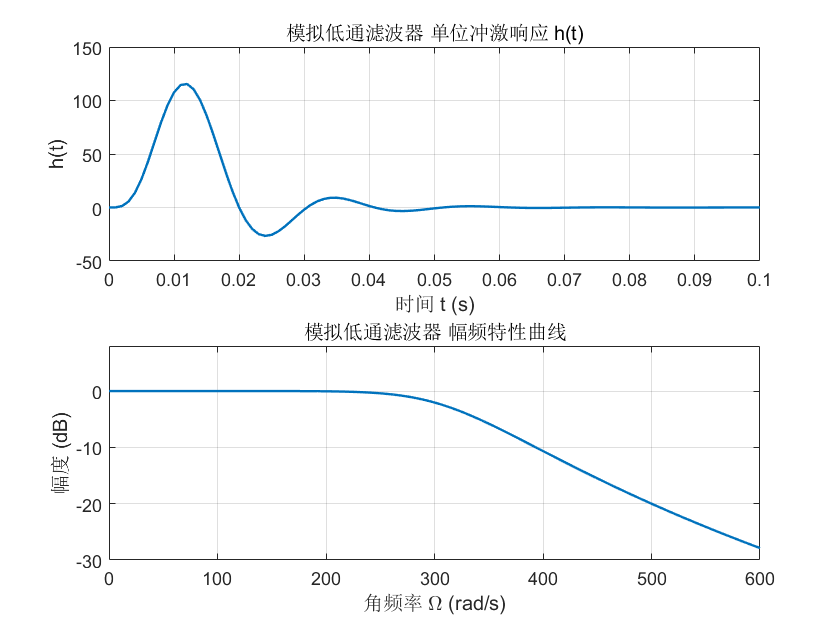
\includegraphics[width=0.9\textwidth]{4.1.png}
\caption{模拟巴特沃斯低通滤波器冲激响应与幅频特性}
\end{figure}

\begin{figure}[H]
\centering
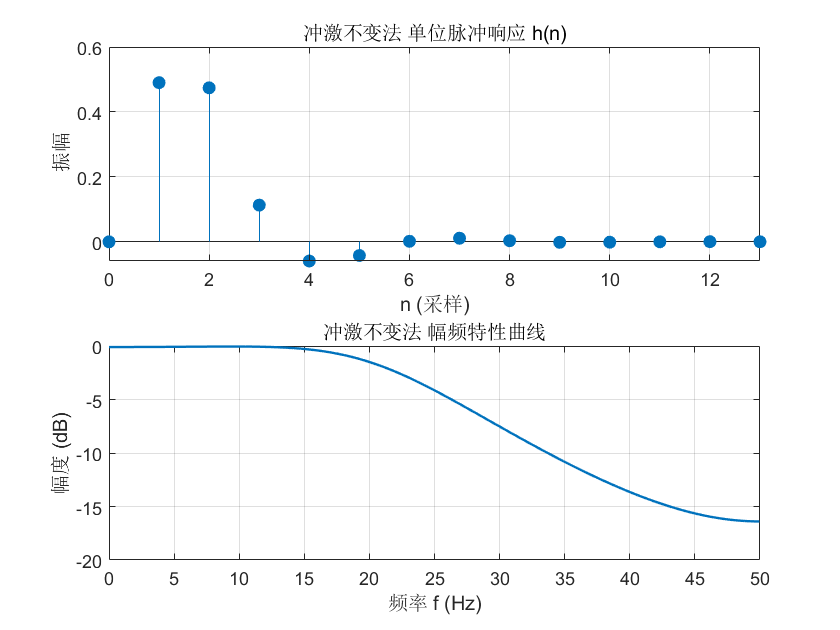
\includegraphics[width=0.9\textwidth]{4.2.png}
\caption{冲激响应不变法数字滤波器脉冲响应与幅频特性}
\end{figure}

\begin{figure}[H]
\centering
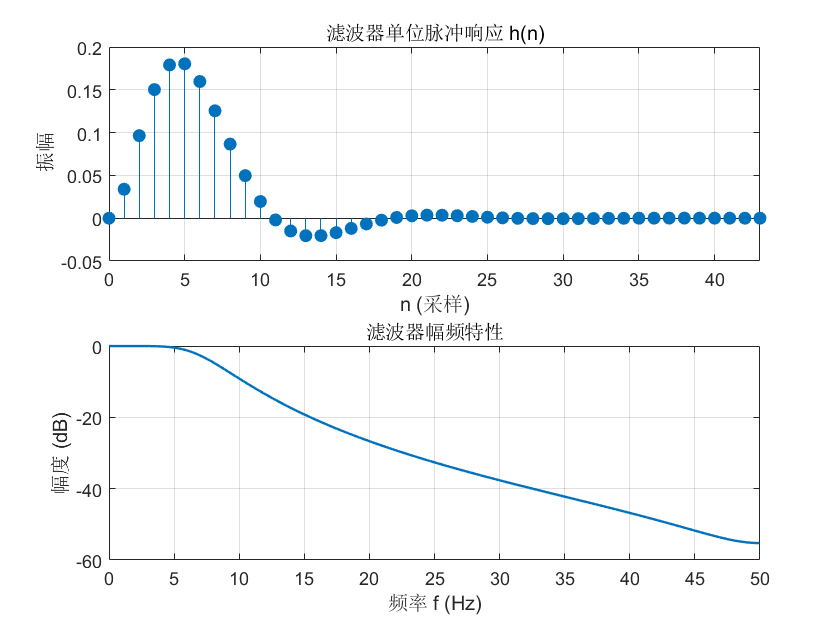
\includegraphics[width=0.9\textwidth]{4.3.png}
\caption{双线性变换法数字滤波器脉冲响应与幅频特性}
\end{figure}

\subsection{五、实验结论}
1. 模拟巴特沃斯滤波器幅频特性通带内平坦无波纹，阻带单调衰减，阶数由通带、阻带衰减指标唯一确定；时域冲激响应收敛稳定，符合因果系统要求。
2. 冲激响应不变法实现模拟到数字滤波器线性频率映射，无频率畸变，但高频存在频谱混叠，仅适用于低通滤波器；数字滤波器脉冲响应随时间衰减收敛。
3. 双线性变换法通过预畸变校正消除频率畸变，无频谱混叠，可设计任意类型滤波器；低频段两种方法滤波效果一致，高频段特性出现明显差异。
4. 仿真得到的幅频特性完全满足预设通带、阻带衰减指标，滤波器设计达标。

\subsection{六、完整MATLAB实验代码}
\subsubsection{exp4\_1.m 模拟巴特沃斯低通滤波器设计}
\begin{lstlisting}
%exp4_1.m 实验四 任务1：模拟巴特沃斯低通滤波器设计
%指标：通带截止300rad/s，阻带截止500rad/s，通带波纹3dB，阻带衰减≥20dB
clear;clc;close all;
%% ==========1. 滤波器性能指标赋值==========
Omega_p = 300;    %模拟通带截止角频率(rad/s)
Omega_s = 500;    %模拟阻带截止角频率(rad/s)
Rp = 3;           %通带最大衰减(dB)
Rs = 20;          %阻带最小衰减(dB)

%% ==========2. buttord求解滤波器最小阶数N、截止临界频率Wn==========
%带's'代表模拟滤波器设计
[n,Wn] = buttord(Omega_p,Omega_s,Rp,Rs,'s');
fprintf('模拟巴特沃斯滤波器阶数 n = %d\n',n);
fprintf('模拟滤波器临界截止角频率 Wn = %.2f rad/s\n',Wn);

%% ==========3. butter生成模拟滤波器分子b、分母a系数==========
[b,a] = butter(n,Wn,'s');

%% ==========4. tf构建系统传递函数H(s)，命令行输出==========
sys = tf(b,a);
disp('=========模拟滤波器系统传递函数 H(s)=========');
disp(sys);

% 新增：输出标准多项式分式形式
num_poly = poly2str(b,'s');
den_poly = poly2str(a,'s');
fprintf('\n========= 多项式分式形式 H(s) =========\n');
fprintf('H(s) = \n');
fprintf('        %s\n',num_poly);
fprintf('--------------------------------------------\n');
fprintf('        %s\n',den_poly);

%% ==========5. impulse求解0~0.1s冲激响应h(t)==========
t = 0:0.001:0.1;   %时间轴：步长0.001s，范围0~0.1s
h_t = impulse(b,a,t);

%% ==========6. freqs求解0~600rad/s幅频特性==========
f_axis = 0:1:600;  %频率轴范围0~600rad/s
[H_s,freq] = freqs(b,a,f_axis);
mag_dB = 20*log10(abs(H_s)); %幅度转换为dB

%% ==========7. 分2行绘图：冲激响应+幅频特性==========
figure('Name','exp4_1 模拟低通滤波器');
%子图1：时域冲激响应
subplot(2,1,1);
plot(t,h_t,'LineWidth',1.2);
title('模拟低通滤波器 单位冲激响应 h(t)');
xlabel('时间 t (s)');
ylabel('h(t)');
grid on;

%子图2：频域幅频特性，约束坐标axis([0 600 -30 8])
subplot(2,1,2);
plot(f_axis,mag_dB,'LineWidth',1.2);
title('模拟低通滤波器 幅频特性曲线');
xlabel('角频率 \Omega (rad/s)');
ylabel('幅度 (dB)');
axis([0 600 -30 8]); %严格遵照指导书坐标轴范围
grid on;
\end{lstlisting}

\subsubsection{exp4\_2.m 冲激响应不变法设计数字低通滤波器}
\begin{lstlisting}
%exp4_2.m 冲激响应不变法设计巴特沃斯数字低通，严格匹配本题指标
clear;clc;close all;
%% 1. 参数设置（严格按题目给定）
Fs = 100;    %采样频率Hz
T = 1/Fs;
wp = 0.4*pi;    %数字通带截止角频率 rad
ws = 0.8*pi;    %数字阻带截止角频率 rad
Rp = 3;      %通带最大衰减dB
Rs = 15;     %阻带最小衰减dB

%% 2. 数字角频率转模拟角频率 Ω=ω/T（冲激响应不变法线性映射）
Omega_p = wp / T;
Omega_s = ws / T;

%% 3. buttord求模拟滤波器最小阶数n和截止频率Wn
[n, Wn] = buttord(Omega_p, Omega_s, Rp, Rs, 's');
fprintf('模拟巴特沃斯原型阶数 n = %d\n',n);

%% 4. butter设计模拟低通H(s)
[b_s, a_s] = butter(n, Wn, 's');

%% 5. impinvar做s→z变换得到数字滤波器系数
[bz, az] = impinvar(b_s, a_s, Fs);

%% 6. tf生成离散系统传递函数H(z)
sys_z = tf(bz, az, T);
disp('=====数字滤波器系统函数H(z)=====');
disp(sys_z);
% 输出分式形式方便报告抄写
num_p = poly2str(bz,'z');
den_p = poly2str(az,'z');
fprintf('\nH(z)分式形式：\nH(z) = %s / (%s)\n',num_p,den_p);

%% 7. 分2行绘图：脉冲响应 + 幅频特性
figure('Name','冲激响应不变法数字低通滤波器');
% 子图1：impz绘制脉冲响应
subplot(2,1,1);
impz(bz,az);
title('滤波器单位脉冲响应 h(n)');
grid on;

% 子图2：freqz求频响，横轴转Hz、纵轴转dB
subplot(2,1,2);
[H, w] = freqz(bz, az, 1024); %w范围0~π归一化角频率
mag_dB = 20*log10(abs(H));
f_Hz = w/(2*pi)*Fs; % 归一化角频率→真实频率Hz
plot(f_Hz, mag_dB, 'LineWidth',1.2);
title('滤波器幅频特性');
xlabel('频率 f (Hz)');
ylabel('幅度 (dB)');
grid on;
\end{lstlisting}

\subsubsection{exp4\_3.m 双线性变换法设计数字低通滤波器（含预畸变）}
\begin{lstlisting}
%exp4_3.m 双线性变换法 带频率预畸变设计数字低通滤波器
clear;clc;close all;
Fs = 100;
T = 1/Fs;
wp = 0.4*pi;
ws = 0.8*pi;
Rp = 3; Rs = 15;

%% 频率预畸变校正
Omega_p = (2/T)*tan(wp/2);
Omega_s = (2/T)*tan(ws/2);

%% 设计模拟原型滤波器
[n,Wn] = buttord(Omega_p,Omega_s,Rp,Rs,'s');
[b_s,a_s] = butter(n,Wn,'s');

%% 双线性变换 s->z
[bz,az] = bilinear(b_s,a_s,Fs);

%% 输出传递函数
sys_z = tf(bz,az,T);
disp('=====双线性变换法 H(z)=====');
disp(sys_z);

%% 绘图
figure('Name','双线性变换法数字低通');
subplot(2,1,1);
impz(bz,az);
title('单位脉冲响应 h(n)');
grid on;

subplot(2,1,2);
[H,w] = freqz(bz,az,1024);
mag_dB = 20*log10(abs(H));
f_Hz = w/(2*pi)*Fs;
plot(f_Hz,mag_dB,'LineWidth',1.2);
title('幅频特性曲线');
xlabel('频率 f(Hz)');
ylabel('幅度(dB)');
grid on;
\end{lstlisting}

\end{document}